\documentclass[a4paper, 12pt, twoside, chapterprefix]{report}

% imports
% =============================================================================
\usepackage{biblatex}
% \usepackage[citestyle=authoryear]{biblatex}
\usepackage{chemformula}
\usepackage{caption}
%\usepackage[superscript,biblabel]{cite}  % not compatible with biblatex
\usepackage{endnotes}
\usepackage{fancyhdr}
\usepackage[left=1.5cm, right=1.5cm, top=2.5cm, bottom=1.5cm]{geometry}
\usepackage{graphicx}
\usepackage[hidelinks]{hyperref}
\usepackage[utf8]{inputenc}
\usepackage{sectsty}      % ?
\usepackage{siunitx}
\usepackage{subfig}
\usepackage{tikz}
\usepackage{xcolor}


% path definitions
% =============================================================================
\addbibresource{references.bib}
\graphicspath{{../figures/}}

% command definitions
% =============================================================================
% author name
\newcommand{\theauthor}{Vincent C. Mader}
% width of line underneath header
\renewcommand{\headrulewidth}{2pt}
% redefine \vec command to have bold vectors
\let\vec\mathbf
% define text color commands
\newcommand{\red}[1]{\textcolor{red}{#1}}
\newcommand{\green}[1]{\textcolor{green}{#1}}
\newcommand{\blue}[1]{\textcolor{blue}{#1}}
% redefine paragraph to include newline after headline
\newcommand{\myparagraph}[1]{\paragraph{#1}\mbox{} \\}


% various 
% =============================================================================
\sisetup{separate-uncertainty}
% treat references as regular section
\defbibheading{secbib}[References]{% 
  \section{#1}%
  % \markboth{#1}{#1}
}
% make font size for chapters large
\chapternumberfont{\Large} 
\chaptertitlefont{\Large}
% Redefine the \chapter* header macro to remove vertical space
\begingroup
\makeatletter
\def\@makeschapterhead#1{% 
  %\vspace*{50\p@}% Remove the vertical space
  {\parindent \z@ \raggedright
    \normalfont
    \interlinepenalty\@M
    \Large \bfseries  #1\par\nobreak
    \vskip 40\p@
  }}
\makeatother

\fancypagestyle{NoHeader}{%
    \fancyhead{}
    \renewcommand{\headrulewidth}{0pt}
}


% document 
% =============================================================================
\begin{document}
  
    % title page
    \pagenumbering{gobble}  % no page numbering (turn back on after title page)
    \newpage
    % \thispagestyle{NoHeader}
    
\begin{titlepage}
  \begin{center}
     
    \Large\textbf{
      Department of Physics and Astronomy\\
      University of Heidelberg
    }
    
    \vspace{18cm}
    
    \normalsize
    Bachelor Thesis in Physics\\
    submitted by\\
    \vspace{0.5cm}
    \Large\textbf{\theauthor}\\
    \normalsize
    \vspace{0.5cm}
    born in Ulm (Germany)\\
    \vspace{0.5cm}
    \Large\textbf{March 2020}
    \normalsize
    
    \newpage\null\thispagestyle{empty}\newpage
    
    \Large\textbf{
      The effect of a Jupiter-sized planet's accretion rate on the
      eccentricity of its orbit
    }
    
    \vspace{18cm}
    
    \normalsize
    This Bachelor Thesis has been carried out by \theauthor\ at the\\
    Max Planck Institute for Astronomy in Heidelberg\\
    under the supervision of\\
    Dr. Bertram Bitsch
    
    \vfill
  \end{center}

\end{titlepage}


  
    % abstract in both English and German
    \newpage
    % \thispagestyle{NoHeader}
    
\section*{Abstract}


    \vspace{30px}
    
\section*{Zusammenfassung}
  Bei der Modellierung von protoplanetaren Scheiben werden häufig numerische 
  Algorithmen verwendet, um die zur Entstehung von Planeten beitragenden 
  Prozesse zu simulieren. Hierzu ist es notwendig, eine Akkretionsroutine
  zu formulieren, die die Ansammlung von Gas auf Planeten in der Scheibe 
  beschreibt. Herkömmlicherweise wird die Akkretionsrate meist unabhängig von 
  der Exzentrizität des Planetenorbits berechnet
  (e.g. \citeauthor{Ida_2018} \citeyear{Ida_2018}, \citeauthor{Benz_2014} 
  \citeyear{Benz_2014} and \citeauthor{Mordasini_2012} 
  \citeyear{Mordasini_2012}).
  . \\
  \\
  In dieser Bachelorarbeit wird ein vereinfachtes Modell einer protoplanetaren 
  Scheibe mithilfe des \textit{FARGO2D1D}-Codes aufgebaut, mit dem Studien zu 
  verschiedenen Parametern von Scheibe und Planeten durchgeführt werden. 
  Ziel ist es zu zeigen, 
  dass die Exzentrizität des Orbits eine große Rolle für die 
  Gas-Akkretionsrate auf einen Planeten spielen kann. Dies liegt daran, dass 
  exzentrische Planeten durch den Austausch von Drehimpuls mit der Scheibe 
  eine deutlich breitere Lücke erzeugen, als es bei einem zirkulären 
  Orbit der Fall wäre. Diese Lücke in der Scheibe ist dementprechend 
  weniger tief, was zur Folge hat, dass die Gasdichte innerhalb der Hill-Sphäre 
  des Planeten deutlich höher ist. Der Planet hat somit mehr Material in seiner
  direkten Umgebung und die Akkretionsrate steigt an. \\
  \\
  Planeten auf elliptischen Orbits erhalten ihre Exzentrizität meist 
  auf eine von zwei Arten: entweder, wenn der Planet massiv genug ist,
  durch Interaktion mit der Scheibe oder durch gravitative Wechselwirkung
  zwischen mehreren Planeten während der Gas-Phase. In beiden Fällen kann ein 
  solcher Planet deutlich schneller akkretieren als ein Planet auf einem 
  zirkulären Orbit. Zukünftige Studien sollten dies berücksichtigen,
  insbesondere bei N-body-Simulationen, bei denen die Exzentrizität schon 
  während der Gas-Phase auftreten kann.
  % Eccentric orbits of giant planets can be generated by two ways: either by 
  % massive planets that interact with their disk or by gravitational 
  % interactions between several planets during the gas phase. This 
  % study shows that if either is the case, planets on eccentric orbits can 
  % accrete gas faster than planets on circular orbits due to the less depleted 
  % planetary gap. Future simulations, especially N-body simualtions where 
  % eccentricities can already arise during the gas phase, need to take these 
  % effects into account.
  %
  % Um ein möglichst genaues Modell für die Akkretionsprozesse innerhalb 
  % protoplanetarer Scheiben zu formulieren, könnte es deshalb von Vorteil sein, 
  % diese Abhängigkeit mit in die Akkretionsroutine aufzunehmen. Dies gilt vor 
  % Allem dann, wenn Systeme um 
  % junge Sterne betrachtet werden, in denen die durchschnittliche Exzentrizität 
  % noch deutlich höher ist als in unserem Sonnensystem.
  % \red{reformulieren}

  
    % preface & acknowledgements
    \newpage
    % \thispagestyle{NoHeader}
    
%\section*{Preface}


    \newpage
    % \thispagestyle{NoHeader}
    
\section*{Acknowledgements}


  
    % table of contents & figures
    \newpage
    \begingroup
      \pagestyle{plain}
      \tableofcontents
      \vspace{300px}
      \listoffigures
      \let\LaTeXStandardClearpage\clearpage
      \let\clearpage\relax  % Do nothing when a \clearpage command appears
      \vspace{50px}
      \listoftables
      \let\clearpage\LaTeXStandardClearpage % Return to the old definition
    \endgroup
  
    % header
    % ---------------------------------------------------------------------------
    \pagestyle{fancy}
    \renewcommand{\chaptermark}[1]{\markboth{#1}{#1}}
    \lhead{Gas Accretion Onto Eccentric Planets}
    \chead{}
    \rhead{\chaptername\ \thechapter\ --\ \leftmark}
  
    % introduction
    
\chapter{Introduction}


  
    % methods
    \newpage
    \chapter{Methods}

  \section{The \textit{FARGO2D1D} Algorithm}
    \label{sec:fargo_algorithm}
    The \textit{FARGO} algorithm was originally introduced by 
    \citeauthor{Masset_1999} (\citeyear{Masset_1999}).
    % Frederic Masset 
    % (1999).
    %"\textit{FARGO}: a fast eulerian transport algorithm for differentially 
    %rotating disks" 
    % \cite{fargo_paper_1999}. 
    The algorithm's name is an acronym for 
    \textit{Fast Advection in Rotating Gaseous Objects}. It is
    written in \textit{C} and utilizes 
    a 5th order \textit{Runge-Kutta} subroutine to determine the trajectory of 
    a planet in the disk, as well as a fluid dynamics subroutine for the gas.
    It is possible to configure whether the planet should interact only with 
    its parent star or also with the gas in the disk, allowing for simulations 
    of planet migration. The gas feels the gravitational potential of the 
    star and the planet. Accretion of gas onto the planet is handled in a 
    simplified way, which will be discussed over the next few paragraphs.
    % \red{(what advantages relative to other methods?)} 
    \\
    \\
    To model a protoplanetary disk, it is represented in the code simply
    by a 2D grid. Each grid cell stands for a specific location in the disk. 
    The row and column of such a cell correspond to its radial and azimuthal 
    position. \\
    \\
    In this thesis, an extension of the standard version of \textit{FARGO} is 
    utilized, titled \textit{FARGO2D1D}. 
    Here, the 2D grid is surrounded by an additional, one-dimensional grid made 
    up of elementary 
    rings. The planet is placed within the 2D section of the grid.
    Far from the center, the gravitational influence of the planet on 
    the structure of the disk is diminishingly small
    \cite{fargo2D1D_what_is_fargo2D1D}. Because of this, the 
    disk can be assumed to be axisymmetric for both very small and very large 
    values of $r$.
    \begin{figure}[h!]
      \centering
      \includegraphics[width=.4\textwidth]{fargo2D1D_grid.png}
      \caption{
        Sketch of the grid that is being used by the \textit{FARGO2D1D} algorithm 
        \cite{fargo_2D1D_grid}. It consists of both a one-dimensional section
        and a two-dimensional section. In the latter, the planet is placed.
      }
    \end{figure}
%    The following paragraphs will \red{attempt to shortly summarize the most
%    important aspects of the algorithm's inner workings}. 

    % \begin{itemize}
    %   \item model of two-dimensional, non-self-gravitating protostellar 
    %     accretion disk
    %   \item embedded: $\sim$ Jupiter-sized protoplanet on an orbit \red{(ecc.?)}
    %   \item goal: solve hydrodynamical equations (Navier-Stokes)
    %   \item \textit{FARGO2D1D} n-body solver for planet motion
    %   \item $+$ accretion \red{how exactly? taken from inside Roche lobe? (for Kley yes)} \\
    %     \red{what function determines the accretion?}
    %   \item \red{different values of $H/r$, $\alpha_{visc.}$}
    % \end{itemize}
    % \red{
    %   parameters $G=1, M_\odot=1, R_0=1$ \\
    %   disk is modeled partially as a 2D array, partially as a 1D array \\
    %   $\Rightarrow$ make plot showing this (look in \textit{FARGO} documentation?)
    % }
 
    \newpage \noindent
    The algorithm in principle allows to have multiple planets in a single disk,
    all interacting with each other as well as with the disk. In this thesis 
    though,
    only a single planet is inside the disk at any given time. At $t=0$, the 
    disk's surface density profile is initialized according to 
    \autoref{eq:surface_density_as_fct_of_r}.
    In the following time steps the planet is introduced to the disk. \\
    \\
    To prevent disruptive shocks or numerical artifacts from arising at 
    the introduction of the planet to the disk,
    its mass is first set to $0$ and then slowly 
    increased over the next few time steps. This time span will be referenced 
    as \textit{tapering period} hereafter. After the tapering period, the 
    planet's mass then is equal to the inital mass value $m_0$ specified in the 
    configuration files. The planet's intial velocity vector is set up in 
    such a way as to position it on an orbit around the star, the 
    eccentricity of which can be manually specified. \\
    \\
    To give the disk some time to settle into an equilibrium state, 
    accretion does not start directly after the tapering has finished.
    Instead, the accretion subroutine is deactivated for a time span that 
    shall be called \textit{accretion wait}. \\
    % The planet is already in orbit 
    % around its star during both the tapering and the accretion wait period. \\
    % TODO: talk about ghost cells?
    \\
 %   % \subsection{Runge-Kutta Subroutine for Planet Motion}
 %   \myparagraph{Runge-Kutta Subroutine For Planet Motion}
 %     \begin{itemize}
 %       \item n-body solver with 5th order Runge-Kutta algorithm
 %       \item family of implicit and explicit iterative methods
 %       \item developed around 1900 by German mathematicians Carl Runge and
 %         Wilhelm Kutta
 %       \item include the well-known routine called the Euler Method
 %     \end{itemize}
 %
 %   % \subsection{Fluid Dynamics Subroutine for Gas Flow}
 %   \myparagraph{Fluid Dynamics Subroutine For Gas Flow}
 %   \red{describe}
 %   
 %   % \subsection{Subroutine for Gas Accretion onto Planet}
 %   \myparagraph{Subroutine For Gas Accretion Onto Planet}
 %     \begin{itemize}
 %       \item uses both Kley and Machida
 %     \end{itemize}
    After the period of accretion wait is over, the planet can finally 
    start gathering mass. This is realized in the code by an accretion
    subroutine, which consists of two parts. Both the \textit{Kley} 
    and \textit{Machida} accretion rates, which will be explained in 
    detail below, are calculated at each time step.
    Afterwards, the minimum value of these two is used to determine 
    the amount of mass removed from the disk and added to the planet.
%    \begin{equation}
%      \dot{m}=\textnormal{max}(\dot{m}_{Kley};\ \dot{m}_{Machida})
%    \end{equation}

    \subsection{Accretion Mechanisms}
      To simulate gas accretion onto a planet, the following approach is used:
      After each time step $\Delta t$, a mass amount $\Delta m$ is 
      removed from the grid cells inside the Hill sphere and added to 
      the planet. % \cite{cite from code}.
      \begin{equation}
        m_{disk}(t+\Delta t)=m_{disk}(t)-\Delta m
      \end{equation}
      \begin{equation}
        m_{planet}(t+\Delta t)=m_{planet}(t)+\Delta m
      \end{equation}
      The precise value of $\Delta m$ is determined by making use of two 
      different models, namely a slightly modified 
      % taking the minimum of 
      % two amounts of mass arrived at by different models. 
      version of both the accretion recipe given by 
      \citeauthor{Kley_1999} (\citeyear{Kley_1999})
      as well as the one given by \citeauthor{Machida_2010}
      (\citeyear{Machida_2010}).
      Both accretion rates are calculated in each timestep,
      then the minimum of these two values is used.
      \begin{equation}
        \Delta m = \textnormal{min}\bigg(
        \Delta m_{Kley};\ 
        \Delta m_{Machida}\bigg)
      \end{equation} \ \\

      \paragraph{Machida Accretion} \ \\
      In the code, a variant of the accretion formula used by 
      \citeauthor{Machida_2010} (\citeyear{Machida_2010}) is utilized, which 
      was derived from 3D isothermal simulations.
      In each time 
      step, the amount of mass to be removed from the Hill sphere is given by 
      \begin{equation}
        \Delta m_{Machida}=\Sigma(r,t)\cdot H^2\cdot\Omega\cdot \textnormal{min}
        \bigg(0.14;\ 0.83\cdot(r_H/H)^{9/2}\bigg)\cdot\Delta t
        \label{eq:machida_accretion}
      \end{equation}
      % \begin{itemize}
      %   \item mention runaway accretion when $m_{core}<m_{envelope}$
      % \end{itemize}
      % \red{be more detailed?}
      % why even use both mechanisms?

      \newpage
      \paragraph{Kley Accretion} \ \\
        Additionally to the Machida accretion, we will use a modified version 
        of the accretion recipe suggested by 
        % W. Kley in his 1999 paper
        % \textit{Mass Flow and Accretion through gaps in Accretion Discs}
        \citeauthor{Kley_1999} (\citeyear{Kley_1999}). 
        % The actual accretion rate for each time step 
        % is determined by taking the 
        The precise value of $\Delta m$ is determined via
        \begin{equation}
          \Delta m=f_{red}\cdot S_{acc}\cdot\Sigma(r,t)\cdot
          f_{acc}\cdot \Delta t
        \end{equation}
        Here, $S_{acc}$ is the size of the disk surface inside the planet's 
        Hill sphere, $\Sigma(r,t)$ is the gas surface density at a distance 
        $r$ from the planet's center at time $t$.
        With the parameter $f_{acc}$, the overall accretion rate can be tweaked
        and $f_{red}$ determines from where precisely in the Hill sphere 
        mass is removed. The latter is defined as
        \begin{equation}
          f_{red} =
          \left\{
          	\begin{array}{ll}
              \frac{2}{3} & \textnormal{if }r/r_H<0.45 \\
              \frac{2}{3}\cdot\cos^4\bigg(r/r_H-0.45\bigg)
                  & \textnormal{if } 0.45 \leq r/r_H\leq 0.95 \\
          		0 & \textnormal{if } r/r_H>0.9
          	\end{array}
          \right.
        \end{equation}
        A visualization of the $r$-dependence of $f_{red}$ can be seen in
        \autoref{fig:f_red_in_the_hill_sphere}.
        \\
        \\
        \\
        \\
        \\
        \begin{figure}[h!]
          \centering
          \begin{minipage}{.5\linewidth}
            \centering
            \subfloat[$r$-dependence of $f_{red}$]{
              \includegraphics[scale=.8]{hill_sphere_kley_fred_2}
            }
          \end{minipage}%
          \begin{minipage}{.5\linewidth}
            \centering
            \subfloat[Visualization of the value of $f_{red}$ in the grid, the 
              red circle marks the boundaries of the Hill sphere.]{
              \includegraphics[scale=.8]{hill_sphere_kley_fred_1}
            }
          \end{minipage}
          \caption{Smoothing function $f_{red}$ that determines where and how 
            much mass is to be taken by the Kley accretion subroutine out of the 
            planetary Hill sphere at each time step.
          }
          \label{fig:f_red_in_the_hill_sphere}
        \end{figure}
        
        \clearpage
        \subsection{Code Units}
          In astronomy, one often has to deal with large numbers, e.g. the 
          solar mass is $M_\odot\approx\SI{1.989e30}{\kilo\gram}$. 
          % In addition to 
          % making numbers less readable and harder to work with,
          % working with large numbers may also lead to bigger numerical errors 
          % due to round-off errors.
          % This can be mitigate by choosing not to utilize SI units. Instead, a 
          To make things easier, we will utilize a different system
          of measurement units in this theis, which will be
          referenced as \textit{code units} hereafter. \\
          \\
          In this system, the basic measuring unit of mass is that of the sun,
          (i.e. $M_\odot=1$). 
          The mass accretion rate $\dot{m}$ of a planet is measured in solar 
          masses per orbit.
          Spatial lengths are measured in multiples of the 
          average distance between Jupiter and the sun, which in SI units 
          amounts to 
          about \SI{5.2}{\astronomicalunit}. All of the simulated planets in 
          this thesis will initially be positioned at this distance, i.e. 
          $r=1$. \\
          \\
          The mass of the central star is assumed to be much larger than that 
          of the planet. Also, the Newtonian gravitational constant $G$ 
          is set to unity as well. Under these assumptions, the Keplerian 
          angular 
          velocity is simply $\Omega_K=1$ and the period of one orbit of a 
          planet 
          (at $r=1$) around the star is $T=2\pi$. \\
          \\
        \\
        \subsection{Default Parameters}
          If not otherwise specified, the following configuration values will be 
          used by default:
          \begin{table}[h!]
            \begin{center}
              \caption{Default simulation parameters}
              \renewcommand{\arraystretch}{1.3}
              \begin{tabular}{l | l}
                parameter & value \\
                \hline
                aspect ratio $h_r$ & 0.05 \\
                flaring index $\beta$ & 0 \\ 
                surface density $\Sigma(r=0)$ & $3\cdot10^{-4}$ \\
                sigma slope $\gamma$ & 1 \\
                viscosity parameter $\alpha_{visc}$ & $10^{-2}$ \\
  %              Roche smoothing & 0.6 \\
  %              exclude Hill & yes \\
                mass tapering period & 50 orbits \\
                radial resolution $N_{rad}$ & 202 \\
                azimuthal resolution $N_{sec}$ & 456 \\
                lower boudary for 2D grid $R_{min,2D}$ & 0.2 \\
                upper boundary for 2D grid $R_{max,2D}$ & 5 \\
                lower boundary for 1D grid $R_{min,1D}$ & 0.02 \\
                upper boundary for 1D grid $R_{max,1D}$ & 50 \\
  %              eccentricity & 0 \\
  %              \red{skip category called "other"} & \\
  %              $N_{tot}$ & 2500 \\
  %              $N_{interm}$ & 50 \\
  %              time between outputs & $2\pi$
              \end{tabular}
  %            \quad
  %            \begin{tabular}{c | c}
  %              $e_0=e(t=0)$ & 0 \\
  %              $m_0=m(t=0)$ & 0.001 \\
  %              $m_{core,0}$ & 0.0003 \\
  %              accretion factor & 1 \\
  %              acc waiting time & 500 \\
  %            \end{tabular}
            \end{center}
          \end{table} \ \\ 
          With these parameters, we can calculate the total mass of the 
          simulated part of the disk:
          \begin{equation}
            m_{disk}=2\pi\int_{0.02}^{50}\Sigma(r=0)\cdot r^{-\gamma}\cdot 
            dr\approx0.015\ M_\odot
            \label{}
          \end{equation}

  \clearpage
  \section{First Runs}
    To get a general idea for the behavior of simulated disks over time,
    see \autoref{fig:first_runs_0}. Here, a top-down view on 
    the disk is shown, which is visualized in polar coordinates for various 
    times. The color coding corresponds to the value of the the gas surface 
    density on a logarithmic scale.
    The influence of the planet's momentum exchange with the gas is clearly 
    visible in the forming spiral arms and the gap, which grows deeper and wider 
    with time. \\
    \\
    In \autoref{fig:first_runs_0.3}, an analogous plot can be seen, 
    this time for a planet on an eccentric orbit ($e=0.3$). Here, the disk 
    evolvution is more chaotic. The gap formed by the planet is also much wider, 
    which will be discussed in more detail later in this thesis, 
    when the effect of the orbital eccentricity on the structure of the gap and 
    therefore on the accretion rate will be investigated.
%    \begin{itemize}
%      \item one can see influence of the planet's momentum 
%        exchange with the gas
%      \item spiral arms form
%      \item gap forms, grows deeper with time
%      \item short simulations, run locally
%      \item get familiar with cluster, slurm
%      \item play around with initial planet mass and eccentricity
%      \item ratio
%        \begin{equation}
%          h_r=H/R
%        \end{equation}
%        is taken as a constant input of the simulation, which means that $h_r$
%        does not change with radial distance from the star. Here, a value of 
%        $h_r=0.05$ is assumed (typical for protostellar accretion disks
%        having a mass inflow rate of $M\approx10^{-7}M_\odot/yr$,
%        \cite{Kley_1999} (\red{why?}))
%    \end{itemize}
    \\
    \begin{figure}[h!]
      \centering
      \begin{minipage}{.3\linewidth}
        \centering
        \subfloat[after 50 orbits]{
          \includegraphics[scale=.25]{frame_rotation/1.0mj_e.000/polar_1_cropped}
        }
      \end{minipage}%
      \begin{minipage}{.3\linewidth}
        \centering
        \subfloat[after 500 orbits]{
          \includegraphics[scale=.25]{frame_rotation/1.0mj_e.000/polar_10_cropped}
        }
      \end{minipage}%
      \begin{minipage}{.3\linewidth}
        \centering
        \subfloat[after 2500 orbits]{
          \includegraphics[scale=.275]{frame_rotation/1.0mj_e.000/polar_50_cropped}
        }
      \end{minipage}
      \caption{
        Evolution of gas surface density over time for a non-migrating,
        non-accreting planet of initial mass $m_0=1\ M_{jupiter}$ 
        on a circular orbit. The disk parameters are 
        $\alpha_{visc}=10^{-2},\ h_r=0.05$. 
        The exchange of angular momentum between gas and planet can be 
        recognized by the formation of a gap in the disk.
      }
      \label{fig:first_runs_0}
    \end{figure}
    \begin{figure}[h!]
      \centering
      \begin{minipage}{.3\linewidth}
        \centering
        \subfloat[after 50 orbits]{
          \includegraphics[scale=.25]{frame_rotation/1.0mj_e.300/polar_1_cropped}
        }
      \end{minipage}%
      \begin{minipage}{.3\linewidth}
        \centering
        \subfloat[after 500 orbits]{
          \includegraphics[scale=.25]{frame_rotation/1.0mj_e.300/polar_10_cropped}
        }
      \end{minipage}%
      \begin{minipage}{.3\linewidth}
        \centering
        \subfloat[after 2500 orbits]{
          \includegraphics[scale=.275]{frame_rotation/1.0mj_e.300/polar_50_cropped}
        }
      \end{minipage}
      \caption{
        Evolution of gas surface density over time for a non-migrating,
        non-accreting planet of initial mass $m_0=1\ M_{jupiter}$ 
        on an elliptic orbit of eccentricity $e_{planet}=0.3$. 
        The disk parameters are 
        $\alpha_{visc}=10^{-2},\ h_r=0.05$. 
        The exchange of angular momentum between gas and planet can again be 
        recognized by the formation of a gap in the disk, which is more wide 
        than in the case of a circular orbit. The gap itself also possesses an 
        eccentricity $e_{gap}\neq0$, 
        which increases both with $e_{planet}$ and $m_0$.
      }
      \label{fig:first_runs_0.3}
    \end{figure}

%    \begin{figure}[h!]
%      \centering
%      \includegraphics[width=\textwidth]{frame_rotation/5mj_e.00/sigma_for_various_times_cropped}
%      \caption{
%        evolution of gas surface density over time  
%        ($m_0=5\ M_{jupiter},\ e_0=0$)
%      }
%    \end{figure} \ \\ 
%
%    \begin{figure}[h!]
%      \centering
%      \includegraphics[width=\textwidth]{frame_rotation/1mj_e.100/sigma_for_various_times_cropped}
%      \caption{
%        evolution of gas surface density over time 
%        ($m_0=1\ M_{jupiter},\ e=0.1$)
%      }
%    \end{figure} \ \\ 
  
  \newpage
  \section{Choosing the Resolution of the 2D Grid}
    The \textit{FARGO2D1D} algorithm defines the resolution of the 2D grid via 
    the two variables $N_{rad}$
    and $N_{sec}$, which designate the number of grid cells in radial and 
    azimuthal direction, respectively. To find the optimal simulation 
    resolution, a compromise has to be found between the integration time and 
    the accuracy of the simulation results. 
    Before this is done though, the optimal ratio between the radial resolution 
    $N_{rad}$ and the azimuthal resolution $N_{sec}$ has to be found: \\
    \\
    The grid is treated by the algorithm simply as a 2D rectangular matrix. In 
    reality though, the system is of course not rectangular, but circular.
    The projection of the rectangular grid into polar coordinates leads to
    a distortion of the square grid cells. The grid cells that are very close
    to the center as well as those very far away from the center are subject to 
    strong distortions. \\
    \\
    To make sure that the accretion subroutine functions accurately,
    the resolution should be chosen in such a way that the grid cells' shape
    is as close to a square as possible at the radial position of the planet
    (i.e. at $r=1$).
    For that, let's take a look at \autoref{fig:radial grid section}, 
    which visualizes a radial grid section at a distance $r$ from the center. 
    \begin{figure}[h!]
      \centering
      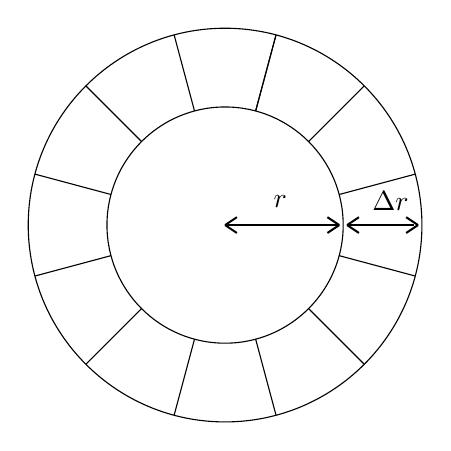
\begin{tikzpicture}

        % circle with segments
        \draw (0, 0) circle (1.5cm);
        \draw (0, 0) circle (2.5cm);
        \foreach \i in {15, 45, 75, 105, 135, 165, 195, 225, 255, 285, 315, 345, 375}
        {
        \draw ({1.5*sin(\i)}, {1.5*cos(\i)}) -- ({2.5*sin(\i)}, {2.5*cos(\i)});
        }

        % left arrow
        \draw [line width=0.25mm, black] (0, 0) -- (1.45, 0);
        \draw [line width=0.25mm, black] (0, 0) -- (0.15, 0.1);
        \draw [line width=0.25mm, black] (0, 0) -- (0.15, -0.1);
        \draw [line width=0.25mm, black] (1.45, 0) -- (1.3, 0.1);
        \draw [line width=0.25mm, black] (1.45, 0) -- (1.3, -0.1);
        \node[] at (0.7, 0.3) {$r$};

        % right arrow
        \draw [line width=0.25mm, black] (1.55, 0) -- (2.4, 0);
        \draw [line width=0.25mm, black] (1.55, 0) -- (1.7, 0.1);
        \draw [line width=0.25mm, black] (1.55, 0) -- (1.7, -0.1);
        \draw [line width=0.25mm, black] (2.45, 0) -- (2.3, 0.1);
        \draw [line width=0.25mm, black] (2.45, 0) -- (2.3, -0.1);
        \node[] at (2.1, 0.3) {$\Delta r$};

      \end{tikzpicture}
      \caption{Sketch of a radial division in the simulation grid}
      \label{fig:radial grid section}
    \end{figure} \ \\ 
    To be as close to a square as possible, each azimuthal ring division should 
    ideally have an area of 
    \begin{equation}
      A_{cell}\approx\Delta r^2
    \end{equation}
    % After the radial boundaries of the grid $r_{min}$ and $r_{max}$ have been 
    % chosen, the width of such a ring can be determined easily for any given 
    % number of radial grid divisions $N_{rad}$ via
    The total area of the ring is given by 
    \begin{equation}
      A_{ring}=\pi(r+\Delta r)^2-\pi r^2=\pi(2r\Delta r+\Delta r^2)
    \end{equation}
    Utilizing the relation $N_{sec}=A_{ring}/A_{cell}$ and then plugging 
    in $r=1$, this yields
    \begin{equation}
      N_{sec}=\pi\bigg(\frac{2}{\Delta r}+1\bigg)
      \label{eq:azimuthal resolution from radial resolution and boundaries}
    \end{equation}
    The width of the ring $\Delta r$ can be determined from the 
    radial resolution and boundaries via
    % $N_{rad}$ via
    \begin{equation}
      \Delta r=\frac{r_{max}-r_{min}}{N_{rad}}
      \label{eq:delta_r_from_bounds_and_n_rad}
    \end{equation}
    % Here, $r_{min}$ and $r_{max}$ denote the inner and outer radial boundaries 
    % of the 2D grid, which are set to $r_{min}=0.2$ and $r_{max}=5$
    % throughout this thesis. 
    It should now be clear how to easily calculate the optimal value of 
    $N_{sec}$ for any value of $N_{rad}$. 
    Still, a few test simulations need 
    to be run before one can decide on the resolution which optimizes the 
    trade-off between integration time and accuracy. 
    % In \textit{SI} units, this outer limit 
    % corresponds to about 26 AU.
    % , as already mentioned.
    % With this, the optimal azimuthal resolution can be calculated easily for
    % any value of $N_{rad}$. as well as the radial boundaries $r_{min}$ and 
    % $r_{max}$ via

    \clearpage \noindent
    % \red{The results of this can be seen in 
    % \autoref{fig:testing cells per rH} and
    % \autoref{fig:testing cells per rH zoomed}}.
    To get a sense of the resolution's influence on the accuracy of the 
    results, simulations are to be run 
%    with an integration time of 500 orbits 
    for multiple different resolutions, namely $2.5,$ $5$ and $10$ cells 
    per Hill radius. For each number $N_{c/rH}$ of cells per Hill radius, 
    $N_{rad}$ can be calculated via 
    \begin{equation}
      N_{rad}=N_{c/rH}\cdot\frac{r_{max}-r_{min}}{r_H}
    \end{equation}
    From this, $N_{sec}$ can be determined with 
    \autoref{eq:azimuthal resolution from radial resolution and boundaries}
    and \autoref{eq:delta_r_from_bounds_and_n_rad}. This yields:
%    This leads to the following values for the radial and azimuthal 
%    resolutions:
    \begin{table}[h!]
      \begin{center}
        \caption{
          Resolutions values for various numbers of 
          grid cells per Hill radius for $m_{planet}=1\ M_{jupiter}$
        }
        \begin{tabular}{c c c}
          cells per $r_H$ & $N_{rad}$ & $N_{sec}$	\\
          \hline 
          2.5 & 101 & 230 \\
          5 & 202 & 456 \\
          10 & 404 & 909 \\
        \end{tabular}
      \end{center}
    \end{table} \ \\
    \autoref{fig:hill_sphere_for_various_resolutions} visualizes how the 
    planet's Hill sphere is implemented in the 2D array. For the simulations,
    a planet on a circular orbit with an intitial mass of $1\ M_{jupiter}$ 
    is used, which builds up during a 
    taper period of 10 orbits. After these 10 orbits, the planet starts
    accreting mass from its surroundings. \\
    \\
    The radial gas density profile after a total of 500 orbits can be seen in 
    \autoref{fig:radial_densities_for_various_resolutions} on the next page.
    There is some 
    discrepancy for small radii, but the overall structure of the gas 
    density profile seems to be pretty much the same. To look at the 
    behavior near zero, 
    \autoref{fig:zoom_in_on_center_of_disk_for_various_resolutions} shows a 
    zoomed in view of the disk. As can be seen here, a resolution of 2.5 
    cells per Hill radius leads to artifacts near the center, which 
    disappear for higher resolution values. \\
    \\
    Since the Hill radius increases with the planet's mass (see 
    \autoref{eq:def_hill_radius}), the number of grid cells inside the Hill 
    radius will grow as time progresses and the planet accretes more 
    material. Thus, these values of $N_{c/r_H}$ only form lower limits and 
    actually get better over time. It has already been shown by
    Lega et al. (2015) that at least 5 cells per Hill radius are necessary 
    to accurately model planet migration.
    % TODO: find out where this is written in the cited paper
    Because this resolution still offers the advantage of faster computation 
    times by a factor of 8
    % \footnote{
    %   One factor 2 in the number of radial cells, one factor 2 in number of 
    %   azimuthal cells and a third factor 2 in the number of time steps due to 
    %   the Courant-Friedrichs-Lewy condition
    % }
    relative to having 10 cells per Hill radius, 
    % Therefore, a resolution of 5 cells per $r_H$ is should lead to 
    % results that accurately show the behavior of the disk and planet within.
%    $\Rightarrow$ mention somewhere that in the end you will have more 
%    grid cells in the Hill radius, because your planet grows! ;)
    all subsequent simulations are run with
    $$N_{rad}=202\textnormal{ and }N_{sec}=456$$
    if not otherwise specified.
%    \red{computation time vs. accuracy, 5 cprH is good enough}
%    \blue{you can also cite here the paper from Lega et al. 2015, who showed 
%    that for migrating planets at least 5 grid cells are needed.}
    \begin{figure}[h!]
      \centering
      \begin{minipage}{.33\linewidth}
        \centering
        \subfloat[$2.5$ cells per $r_H$]{
          \includegraphics[scale=.55]{hill_sphere_2,5_cells.pdf}
        }
      \end{minipage}%
      \begin{minipage}{.33\linewidth}
        \centering
        \subfloat[$5$ cells per $r_H$]{
          \includegraphics[scale=.55]{hill_sphere_5_cells.pdf}
        }
      \end{minipage}%
      \begin{minipage}{.33\linewidth}
        \centering
        \subfloat[$10$ cells per $r_H$]{
          \includegraphics[scale=.55]{hill_sphere_10_cells.pdf}
        }
      \end{minipage}
      \caption{Visualization of Hill spheres in the grid for various resolutions}
      \label{fig:hill_sphere_for_various_resolutions}
    \end{figure}

    \newpage
%    \begin{figure}[h!]
%      \centering
%      \begin{minipage}{\linewidth}
%        \centering
%        \subfloat[zoomed out]{
%          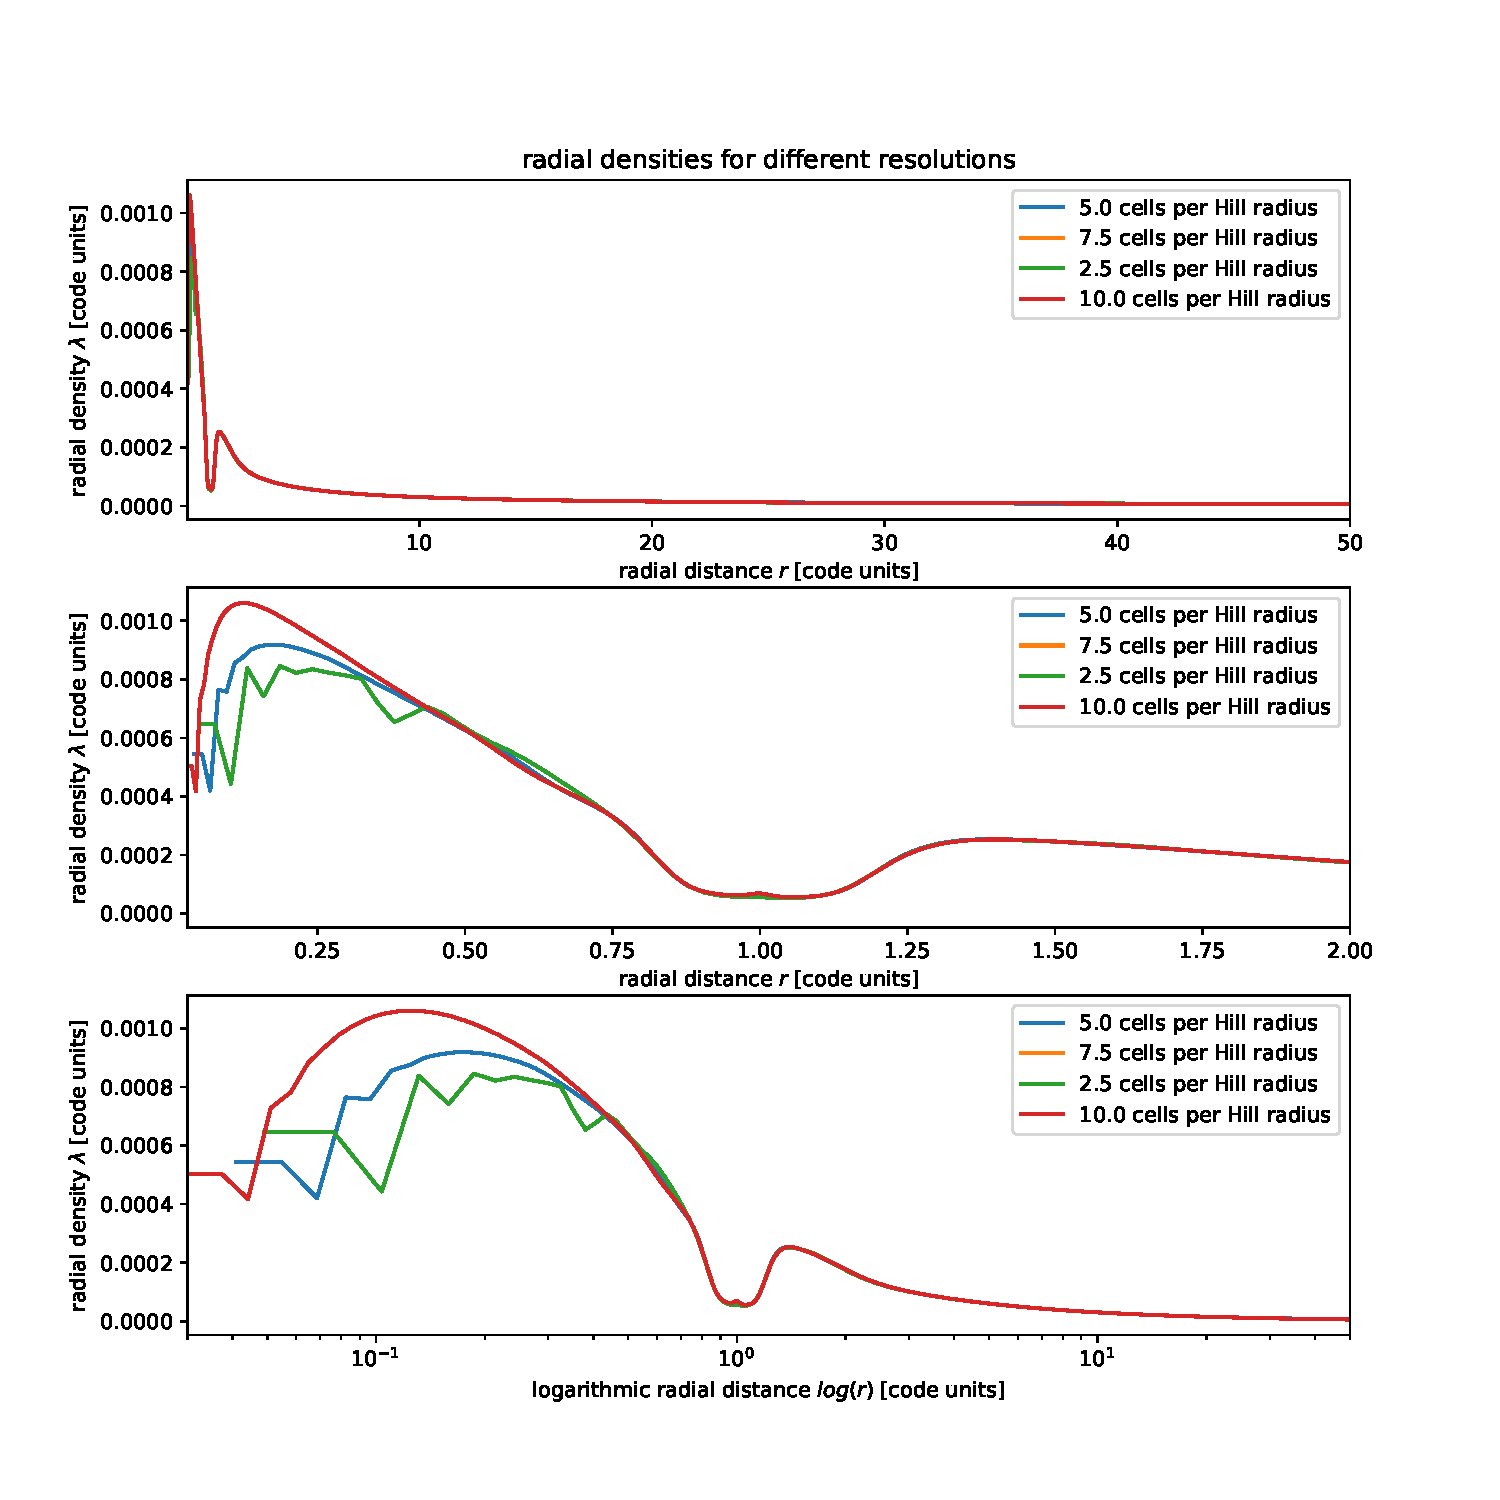
\includegraphics[scale=.8]{testing_cells_per_rH/radial_densities_by_resolution}
%        }
%      \end{minipage} \\
%      \begin{minipage}{\linewidth}
%        \centering
%        \subfloat[zoomed in]{
%          \includegraphics[scale=.8]{testing_cells_per_rH/radial_densities_by_resolution_loglog}
%        }
%      \end{minipage} \\
%      \caption{azimuthally averaged gas densities after 500 orbits for different resolutions}
%    \end{figure} \ \\

    \begin{figure}[h!]
      \centering
      \includegraphics[width=.9\textwidth]{testing_cells_per_rH/radial_densities_by_resolution_loglog}
      \caption{Azimuthally averaged surface densities at $t=500$ orbits for 
        three different grid resolutions. A single planet is positioned at 
        $r=1$. Its mass is initialized to $m_0=1\ M_{jupiter}$ during a tapering
        period of 5 orbits. Accretion starts at $t=10$ orbits.
        Thus, the planet undergoes accretion for a total of 490 orbits.
        The planet is put on a circular orbit, migration is 
        turned off and the disk is characterized by the parameters 
        $\alpha_{visc}=10^{-2}$,\ $h_r=0.05$.
        The general structure of the 
        gas density follows approximately the same course for all resolution 
        values, with discrepancies being the largest for small values of $r$.
      }
      \label{fig:radial_densities_for_various_resolutions}
    \end{figure} \ \\ 

    \begin{figure}[h!]
      \centering
      \begin{minipage}{.3\linewidth}
        \centering
        \subfloat[]{
          \includegraphics[scale=.27]{testing_cells_per_rH/2.5c_per_rH_e.0/polar_10_cropped}
        }
      \end{minipage}%
      \begin{minipage}{.3\linewidth}
        \centering
        \subfloat[]{
          \includegraphics[scale=.27]{testing_cells_per_rH/5c_per_rH_e.0/polar_10_cropped}
        } 
      \end{minipage}%
      \begin{minipage}{.3\linewidth}
        \centering
        \subfloat[]{
          \includegraphics[scale=.28]{testing_cells_per_rH/10c_per_rH_e.0/polar_10_cropped}
        }
      \end{minipage}
      \caption{
        Gas surface density in the inner regions of the 2D grid for 
        different resolutions at $t=500$ orbits. 
        The planet's mass is initialized to $m_0=1\ M_{jupiter}$ during a 
        tapering period of 5 orbits. Accretion starts at $t=10$ orbits.
        Thus, the planet undergoes accretion for a total of 490 orbits.
        The planet is put on a circular orbit and migration is 
        turned off. The disk is characterized by the parameters 
        $\alpha_{visc}=10^{-2}$,\ $h_r=0.05$.
        The black rings indicate the distance from the 
        center, the color bar displays the order of magnitude (decadic 
        logarithm) of the gas density in code units. For the lowest resolution, 
        artifacts can be observed near the center of the disk,
        which disappear at higher resulution. Each doubling of the number 
        of cells per Hill radius leads to a factor 8 increase in the needed 
        computation time. Therefore, in this thesis we focus 
        on simulations that initially have 5 grid cells per Hill radius.
      }
      \label{fig:zoom_in_on_center_of_disk_for_various_resolutions}
    \end{figure}
%    \begin{figure}[h!]
%      \centering
%      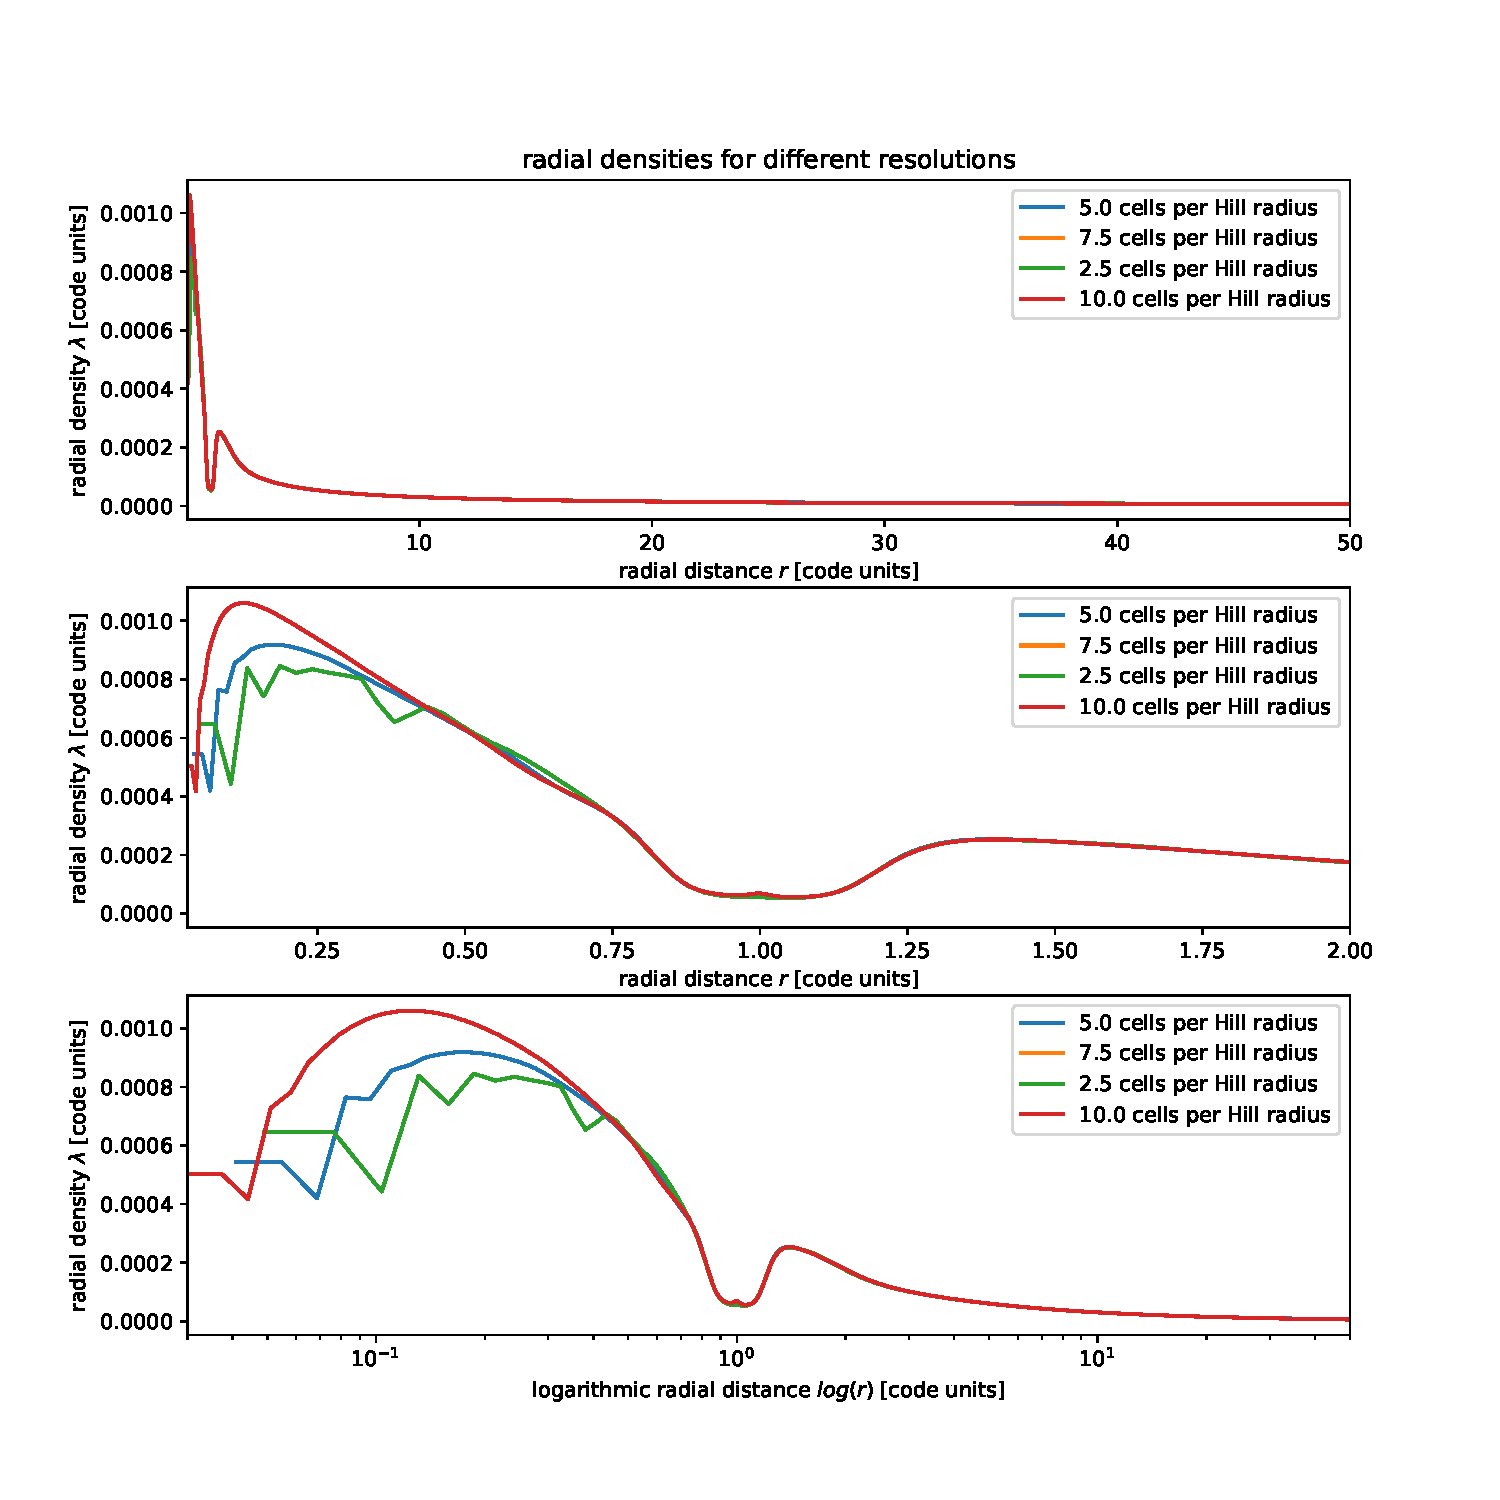
\includegraphics[width=\textwidth]{testing_cells_per_rH/radial_densities_by_resolution}
%      \caption{
%        azimuthally averaged gas densities after 500 orbits for different resolutions}
%      \label{fig:testing cells per rH}
%    \end{figure} \ \\ 
%    \begin{figure}[h!]
%      \centering
%      \includegraphics[width=\textwidth]{testing_cells_per_rH/radial_densities_by_resolution_loglog}
%      \caption{radial densities after 500 orbits for different resolutions}
%      \label{fig:testing cells per rH}
%    \end{figure} \ \\ 
%    To investigate the behavior near the planet, the following plot shows the
%    same data, but this time zoomed in on the gap. 
%    \begin{figure}[h!]
%      \centering
%      \includegraphics[width=\textwidth]{testing_cells_per_rH/radial_densities_by_resolution_zoom}
%      \caption{radial densities after 500 orbits for different resolutions (zoomed in)}
%      \label{fig:testing cells per rH zoomed}
%    \end{figure} \ \\ 


  \newpage
%  \section{Variation of the Parameters of the Protoplanetary Disk}
  \section{Parameter Studies of the Disk}
  
   In this section, we investigate how the gas accretion rate onto the planet 
   as well as the structure of the gap are influenced by the disk's
   characteristics, namely its geometry and the viscosity of the gas within
   the disk.
%  planet's accretion rate and gap structure is investigated. This is 
%  done for the disk's aspect ratio, radial gas profile and gas viscosity.
%  as 
%  well as for the planet's intitial mass, eccentricity and \red{accretion rate}.
 
    \subsection{Disk Geometry}
      \label{sec:disk_geometry}
      In our model, the geometry of the disk is mainly characterized by the 
      aspect ratio $h_r$ as well as the flaring index $\beta$. Let us first 
      take a look at the influence of the aspect ratio. Simulations were 
      carried out for various values of $h_r$ with an integration time of 
      2500 orbits. During the first 50 orbits, the planet mass is slowly 
      increased to $1\ m_{jupiter}$. Accretion starts at $t=500$ orbits.
      The results can be seen in \autoref{fig:varying_aspect_ratio}a,
      where the gas density profile in the vicinity of the planet plotted
      as a function of the distance $r$ from the disk center, and 
      \autoref{fig:varying_aspect_ratio}, where the relative mass increase 
      of the planet is plotted against $h_r$. \\
      \\
      Higher values of the aspect ratio lead to a less deep gap, as has 
      already been stated by \citeauthor{Crida_2006} (\citeyear{Crida_2006}). 
      This is to be expected, since in a thicker disk more material is available 
      and therefore more gas diffuses into the forming gap, hindering the planet 
      from depleting the region. \\
      \\
%      As the gap is shallower for large $h_r$, the accretion rate increases as 
%      well. \\
      One would expect that the accretion rate of the planet increases with
      the amount of gas in its Hill sphere. This is exactly what we see in 
      \autoref{fig:varying_aspect_ratio}b. Thicker disks lead to faster 
      gas accretion onto a planet in the disk. Furthermore, it seems that the 
      relationship between aspect ratio and accretion rate is a linear one,
      at least in this simplified model. \\
      \\
      The influence of the flaring index $\beta$ is of a similar kind. Higher 
      values of $\beta$ lead to a shallower gap and higher accretion rate.
      % Since
      % it determines the slope of the power law describing the gas surface 
      % density as a function $r$ (see \autoref{eq:surface_density_as_fct_of_r}),
      % higher values of $\beta$ correspond to more gas being available for 
      % accretion the vicinity of the planet. \\
      % \blue{careful: think about your normalisations. at r=1 the flaring does not matter}
      % \\
      Interestingly, the curves describing the surface density profile cross 
      each other when varying the aspect ratio, but do not when varying the 
      flaring index. Instead, \autoref{fig:varying_flaring_index} shows what 
      seems to be an additive offset between the gas profiles for different 
      flaring indices. Increasing both $h_r$ and $\beta$ leads to a shallower 
      gap, yet the surface density in disk regions around the gap grows 
      with $\beta$ and falls when increasing $h_r$. \\
      \\
      % \red{
      %   Why is this? 
      % } \\
      % \\
      % This is because $\beta$ increases gas density throughout 
      % the whole disk, while $h_r$ and $\alpha_{visc}$ (where the curves 
      % also cross) accelerate diffusion back into the gap? 
        % Then, the 
        % gap should only get shallower if the surrounding regions lose some of 
        % their material
      % \blue{changing beta does not change the disc density!!!! a change in beta changes the vertical gas distribution, not the total amount \\ \\
      %   correct about $h_r$ and alpha: if they increase your viscosity increases and thus viscous diffusion}
        % \begin{itemize}
          % \item $\beta$ changes the surface density throughout the disk, gap 
          %   less deep because more material available, same amount per time 
          %   moved by planet for each sim
          % \item $h_r$ and $\alpha_{visc}$ changes the rate at which material 
          %   flows into the gap $\Rightarrow$ deeper gaps can only exists when 
          %   the regions around the gap get more material
        % \end{itemize}
%      \begin{itemize}
%        \item gap can't form for large values of $h_r$
%        \item accretion increases linearly with $h_r$, i.e. with disk width \\
%        $\Rightarrow$ makes sense, more material available
%      \end{itemize}
%      \red{why does the flaring index allow for more accretion?
%        $\Rightarrow$ mention in the text that a higher H/r results in a 
%        less deep gap, which is already stated by Crida et al. 2006. The 
%        less deep gap then has more material in the horseshoe region so 
%        you can accrete faster and grow more
%      }

      \newpage
      \begin{figure}[h!]
        \centering
        \begin{minipage}{.5\linewidth}
          \centering
          \subfloat[surface density vs. aspect ratio]{
            \includegraphics[scale=.8]{aspect_ratio/sigma_vs_r_and_hr}
          }
        \end{minipage}%
        \begin{minipage}{.5\linewidth}
          \centering
          \subfloat[increase of mass vs. aspect ratio]{
            \includegraphics[scale=.8]{aspect_ratio/mpm0_vs_hr}
          }
        \end{minipage}
      \caption{
        Influence of the disk's aspect ratio $h_r$ on the gap profile and
        the increase of the planet's mass after an integration time of 2500 
        orbits. The first 50 of these orbits make up the tapering 
        period (afterwards $m_0=1\ M_{jupiter}$) and the planet starts accreting 
        after 500 orbits, the total duration of accretion is
        2000 orbits. The planet is put on a circular orbit and migration is
        deactivated. The disk is characterized by the parameters 
        $\alpha_{visc}=10^{-2}$,\ $h_r=0.05$. 
        A thicker disk leads to more 
        material diffusing into the forming gap, thus stifling its growth 
        while accelerating accretion onto the planet.
        % As one would expect, higher values for the aspect ratio lead to 
        % a less deep gap and thus to faster accretion.
        }
        \label{fig:varying_aspect_ratio}
      \end{figure}

      \begin{figure}[h!]
        \centering
        \begin{minipage}{.5\linewidth}
          \centering
          \subfloat[surface density vs. flaring index]{
            \includegraphics[scale=.8]{flaring_idx/sigma_vs_r_and_flaring_idx}
          }
        \end{minipage}%
        \begin{minipage}{.5\linewidth}
          \centering
          \subfloat[increase of mass vs. flaring index]{
            \includegraphics[scale=.8]{flaring_idx/mpm0_vs_flaring_idx}
          }
        \end{minipage}
      \caption{
        Gap profile and relative planet mass increase as a function of 
        the disk's flaring index after an integration time of 2500 orbits. The 
        first 50 of these orbits make up the tapering 
        period (afterwards $m_0=1\ M_{jupiter}$) and the planet starts accreting 
        after 500 orbits. Thus, the total accretion time has a duration of 
        2000 orbits. The planet is put on a circular orbit and migration is
        deactivated. The disk is characterized by the parameters 
        $\alpha_{visc}=10^{-2}$,\ $h_r=0.05$.
        For higher values of 
        $\beta$, the gap is less deep and the accretion rate increases.
        % Higher values of the flaring index 
        % lead to shallower gaps and faster accretion.
      }
      \label{fig:varying_flaring_index}
      \end{figure} 

%    \clearpage
%    \subsection{Radial Gas Profile \red{(sigma slope)}}
%
%      \begin{itemize}
%        \item
%      \end{itemize}

    \clearpage
    \subsection{Gas Viscosity Parameter}
      Next, we investigate the influence of the gas viscosity parameter 
      $\alpha_{visc}$. The simulations for this study were carried out using 
      the same parameters as used in \autoref{sec:disk_geometry}, only this 
      time the viscosity is not held constant. The aspect ratio is set to 
      $h_r=0.05$. 
      \\
      \\
      In \autoref{fig:influence_of_alpha}a, the gas 
      surface density profile is plotted against the distance from the star.
      Large values of $\alpha_{visc}$ lead to a much less deep gap. While the 
      planet's tidal influence due to gravity leads to a gas depletion in the 
      regions close to its orbit, the material from further in- or outwards 
      diffuses back in. If the gas is very viscous, this happens only slowly,
      and a gap can form. If, on the other hand, $\alpha_{visc}$ is large,
      the gap stays very shallow. \\
      \\
      This is reflected in the relative mass 
      increase that is plotted in \autoref{fig:influence_of_alpha}b. 
      High values of $\alpha_{visc}$ lead to much more material being accreted 
      by the planet, simply because there is that much more gas available 
      in the its vicinity, analogous to what we saw for the parameter 
      studies of the aspect ratio and flaring index. \\
      \\
      A planet introduced to the disk pushes material away from its orbit,
      which then needs to diffuse away. For low values of 
      $\alpha_{visc}$ this takes longer than for high values. This explains the 
      fact that high alpha values lead to larger bump interior and exterior to 
      the planets position.
      \\
      \\
      \\
      \\
%      \begin{itemize}
%        \item accretion increases with $\alpha$, not linear (why)
%        \item gap doesn't form for large $\alpha$
%        \item numerical viscosity \red{(removed the data point for
%          $\alpha_{visc}<10^{-4}$)}
%      \end{itemize}
      \begin{figure}[h!]
        \centering
        \begin{minipage}{.5\linewidth}
          \centering
          \subfloat[surface density vs. viscosity]{
            \includegraphics[scale=.8]{testing_visc/sigma_vs_r_and_viscosity}
          }
          \label{fig:influence_of_alpha:a}
        \end{minipage}%
        \begin{minipage}{.5\linewidth}
          \centering 
          \subfloat[increase of mass vs. viscosity]{
            \includegraphics[scale=.8]{testing_visc/mpm0_vs_visc}
          }
          \label{fig:influence_of_alpha:b}
        \end{minipage}
        \caption{
          Influence of the disk's viscosity parameter $\alpha_{visc}$ on 
          the gap profile as well the relative planet mass increase after an 
          integration time of 2500 orbits. The first 50 of these orbits make up 
          the tapering period (afterwards $m_0=1\ M_{jupiter}$) and the planet 
          starts accreting after 500 orbits. Therefore, the planet undergoes 
          accretion for a total of 2000 orbits. It is initialized on a circular 
          orbit and migration is deactivated. The disk is characterized by the 
          parameters $\alpha_{visc}=10^{-2}$,\ $h_r=0.05$.
          The depth of the gap decreases with the viscosity parameter. Less 
          viscous disks supply a faster inflow of gas into the low density 
          regions created by the planet. Accretion accordingly grows with 
          $\alpha_{visc}$.
        }
        \label{fig:influence_of_alpha}
      \end{figure}

  \newpage
  \section{Parameter Studies of the Planet}
    It would be great to gain insight into how the features of the planet 
    affect its accretion rate. To do this, we first vary the initial mass of 
    the planet after tapering. Afterwards, we take a look at the influence of 
    the eccentricity of the planet's orbit. \\
    \\
    In the code, the accretion rate itself can be tweaked by scaling it up or 
    down by a multiplicative factor. This is investigated as well, to find 
    out how the gap structure and the relative increase in planet mass behave 
    for high rates of gas accretion.

    \subsection{Initial Planet Mass}
      In \autoref{fig:gap_vs_initial_mass}, the structure of the gap is 
      displayed for various different values of the initial planet mass.
      Just as one would expect from earlier investigations by e.g. 
      \citeauthor{Kley_2006} (\citeyear{Kley_2006}), planets with a larger
      mass carve out a deeper 
      gap due to their greater exchange of angular momentum with the gas. \\
      \\
      The opening of the gap of course directly influences the amount of gas in 
      the Hill region of the planet and therefore  its gas accretion rate,
      as can be seen in \autoref{fig:accretion_vs_m0}, where the absolute 
      and relative mass increase is displayed against the initial mass. 
      \autoref{fig:accretion_vs_t_and_m0} shows the mass increase against time.
      \\
      \\
      Relative to their own intital mass, the smaller planets experience 
      the highest accretion rates. \\
      \\
      \\
      % \begin{itemize}
      %   \item smaller planets accrete faster (relative to initial mass) \\
      %   $\Rightarrow$ makes sense, larger planets open gap faster/wider
      % \end{itemize}
      
      \begin{figure}[h!]
        \centering
        \includegraphics[width=.9\textwidth]{frame_rotation/sigma_vs_r_and_m0}
        \caption{
          Surface density as a function of $r$ for various initial planet 
          masses after an integration time of 2500 
          orbits. The first 50 of these orbits make up the tapering 
          period and the planet starts accreting 
          after 500 orbits. Thus, the total accretion time has a duration of 
          2000 orbits. The planet is put on a circular orbit and migration is
          deactivated. The disk is characterized by the parameters 
          $\alpha_{visc}=10^{-2}$,\ $h_r=0.05$.
          Due to their stronger interaction with the disk, high-mass planets
          carve out deeper and wider gaps than low-mass planets.
          }
          \label{fig:gap_vs_initial_mass}
      \end{figure}

      \begin{figure}[h!]
        \centering
        \begin{minipage}{.5\linewidth}
          \centering
          \subfloat[absolute planet mass]{
            \includegraphics[scale=0.8]{frame_rotation/m_vs_m0}
          }
        \end{minipage}%
        \begin{minipage}{.5\linewidth}
          \centering
          \subfloat[relative mass increase $m/m_0$]{
            \includegraphics[scale=0.8]{frame_rotation/mpm0_vs_m0}
          }
        \end{minipage}
        \caption{
          Absolute and relative mass increase of a planet for various 
          initial masses. The total integration time is 2500 orbits, of 
          which the first 50 orbits make up the tapering 
          period and the planet starts accreting 
          after 500 orbits. Thus, the total duration of accretion is
          2000 orbits. The planet is put on a circular orbit and migration is
          deactivated. The disk is characterized by the parameters 
          $\alpha_{visc}=10^{-2}$,\ $h_r=0.05$.
          Low-mass planets experience faster accretion due them creating only 
          small gaps.
        }
        \label{fig:accretion_vs_m0}
      \end{figure} 

      \begin{figure}[h!]
        \centering
        \begin{minipage}{.5\linewidth}
          \centering
          \subfloat[mass increase vs. time and $m_0$]{
            \includegraphics[scale=.8]{frame_rotation/mpm0_vs_t_and_mass}
          }
        \end{minipage}%
        \begin{minipage}{.5\linewidth}
          \centering
          \subfloat[accretion rate vs. time and $m_0$]{
            \includegraphics[scale=.8]{frame_rotation/dotm_vs_t_and_mass}
          }
        \end{minipage}
        \caption{
          Relative mass increase and accretion rate as a function of time for
          different initial planet masses. The integration time is
          2500 orbits, of which the first 50 orbits make up the tapering 
          period, the planet starts accreting 
          after 500 orbits. Thus, the planet experiences accretion for a total 
          2000 orbits. The planet is put on a circular orbit and migration is
          deactivated. The disk is characterized by the parameters 
          $\alpha_{visc}=10^{-2}$,\ $h_r=0.05$.
          Planets accrete the fastest when they're still small, because the 
          gap they create is much more shallow compared to more massive planets.
        }
        \label{fig:accretion_vs_t_and_m0}
      \end{figure} 

      % \clearpage 
      \newpage
      \noindent
      \myparagraph{Gas Surface Density Profile At Time Of Equal Accretion}
      It would be interesting to see what the profile of the gap looks like 
      at times of equal accretion for various planet masses. If the accretion 
      rate is the same, then it would make sense if the amount of gas in the 
      Hill sphere of the planet were similar or the same as well. \\
      \\
      Let us look at points in time at which the accretion rate on a planet 
      is approximately equal to $6\cdot10^{-9}$ solar masses per orbit. 
      \autoref{fig:comparing_gap_for_times_of_equal_acc}a attempts to visualize
      this. The times of interest are at the intersections between the black 
      lines and the time axis. For each of these times, the surface density 
      profile in the vicinity of the planet (divided by the unperturbed 
      profile) is plotted in 
      \autoref{fig:comparing_gap_for_times_of_equal_acc}b. \\
      \\
      % Indeed, the radial gas profile is \red{quite} similar 
      % \red{
      %   (
      %     at least more similar than in 
      %     \autoref{fig:gap_vs_initial_mass}
      %   )
      % }
      The gap profiles are quite similar, which becomes clearer when 
      compared to what we already saw in \autoref{fig:gap_vs_initial_mass}. 
      To define a measure of how similar the gap profiles are for simulations 
      with various planet masses, let us define the depth of the gap as 
      $\Sigma(r=1)$, which can be abbreviated to $\Sigma_0$. At times of 
      approximately equal accretion, the ratio 
      between the depth of the gap formed by a planet with $m=0.5\ m_{jupiter}$ 
      and the gap of a planet with $m=1.5\ m_{jupiter}$ is
      $$\frac{\Sigma_0(m=0.5\ m_{jupiter})}{\Sigma_0(m=1.5\ m_{jupiter})}
      \approx1.5\ \ \ \textnormal{(at times of equal acc. rate)}$$
      while the gas densities shown in \autoref{fig:gap_vs_initial_mass} lead 
      to a ratio of 
      $$\frac{\Sigma_0(m=0.5\ m_{jupiter})}{\Sigma_0(m=1.5\ m_{jupiter})}
      \approx2.2\ \ \ \textnormal{(after 2000 orbits of acc.)}$$
      Thus, the gap profiles appear to indeed be more similar when comparing 
      them at times of equal accretion than when comparing them after a fixed 
      amount of time. That the gap profiles are not perfectly identical may 
      partly be due to the fact that simulation output files were generated 
      only every 50 orbits, so 
      that the accretion rates are not exactly $6\cdot10^{-9}$ solar masses per 
      orbit at these times.
      % \red{plot mass in Hill sphere, similar?}
      \begin{figure}[h!]
        \centering
        \begin{minipage}{.5\linewidth}
          \centering
          \subfloat[mass increase vs. time and $m_0$]{
            \label{:a}
            \includegraphics[scale=.8]{frame_rotation/dotm_vs_t_and_mass_3}
          }
        \end{minipage}%
        \begin{minipage}{.5\linewidth}
          \centering
          \subfloat[gap profile]{
            \label{:b}
            \includegraphics[scale=.8]{frame_rotation/sigma_vs_r_for_same_acc_rates}
          }
        \end{minipage}
        \caption{
          Comparison of gas density profiles at times of equal accretion. 
          From the simulation results already shown in 
          \autoref{fig:accretion_vs_t_and_m0}a, we focus on the planets with 
          the lowest mass, which meet the condition 
          $\dot{m}\approx6\cdot10^{-9}$ solar masses per orbit for 
          different times. The gap profile is plotted for these times of
          equal accretion rates. % TODO: describe, good? bad?
          % \newline
          % \red{
          %   do this again for lower acc rate? 
          %   $\Rightarrow$ more planets to compare
          % }
        }
        \label{fig:comparing_gap_for_times_of_equal_acc}
      \end{figure} \ \\

    \clearpage \noindent
    We can also calculate the mass inside the Hill sphere for each of the 
    simulations. This yields 
    $$m_{Hill}(m=0.5\ m_{jupiter})=5.5\cdot10^{-3}$$
    $$m_{Hill}(m=1.0\ m_{jupiter})=5.6\cdot10^{-3}$$
    $$m_{Hill}(m=1.5\ m_{jupiter})=5.9\cdot10^{-3}$$
    As above, the relative differences between those values are probably 
    explained by the fact that the accretion rate is not exactly the same,
    since outputs were only generated every 50 orbits. Even though the planet 
    with $m=1.5\ M_{jupiter}$ created the deepest gap, it also has the most 
    matter in its Hill sphere. This can be attributed to the fact that the 
    Hill sphere grows with the mass of the planet.
    \subsection{Numerical Accretion Rate}
      Let us take a look at the influence of the accretion rate of gas onto 
      the planet, which can be tweaked in the code. Simulations are run for 
      various factors between 0.5 and 3.0. The results can be seen in 
      \autoref{fig:influence_of_machida}. \\
      \\
      As we increase the factor controlling the accretion rate, the gap grows 
      deeper and the planet's mass increase grows larger, just as one would 
      expect. It is interesting to see though that the relation between the 
      relative mass increase and the accretion factor is not a linear one,
      but that the effect of the accretion factor on the mass increase 
      seems to weaken for high values. 
      This is due to the eventual depletion of the Hill region. The relative 
      mass increase is limited for very high accretion factors by the gas 
      inflow into the gap from regions further in- or outwards, which is set 
      by the disk's viscosity. 
      % \begin{itemize}
      %   \item relative planet mass increase grows with accretion factor
      %     (obviously, makes sense)
      %   \item there is an upper limit, gap forms, horse show region depletes \\
      %     $\Rightarrow$ accretion limited by gas inflow (disk viscosity)
      % \end{itemize}
      \begin{figure}[h!]
        \centering
        \begin{minipage}{.5\linewidth}
          \centering
          \subfloat[radial gas density vs. accretion]{
            \includegraphics[scale=.8]{machida/sigma_vs_r_and_machida}
          }
        \end{minipage}%
        \begin{minipage}{.5\linewidth}
          \centering
          \subfloat[mass increase vs. accretion]{
            \includegraphics[scale=.8]{machida/mpm0_vs_machida}
          }
        \end{minipage}
        \caption{
          Influence of the numerical accretion rate on the gap profile
          and the planet's mass increase after the end of a simulation
          with an integration time of 2500 orbits. The first 50 of these orbits 
          make up the tapering period and the planet starts accreting after 500 
          orbits. Thus, the total accretion time possesses a duration of 
          2000 orbits. The planet is put on a circular orbit and migration is
          deactivated. The disk is characterized by the parameters 
          $\alpha_{visc}=10^{-2}$,\ $h_r=0.05$.
          High accretion rates lead to a large increase in planet mass, 
          obviously. The effect is less noticable for high values of the 
          accretion factor though, because the regions near the planet 
          become more and more depleted and accretion slows down.
        }
        \label{fig:influence_of_machida}
      \end{figure} \ \\

    \clearpage
    \subsection{Initial Planet Eccentricity}
      Up until now, we've almost exclusively investigated planets on circular 
      orbits. Let us now turn our attention towards planets with orbital 
      eccentricities
      $e\neq0$. For the time being, the value of $e$ is configured at the 
      beginning of the simulation and then does not change over time, i.e. 
      migration and eccentricity damping is turned off and the planet 
      does not feel the gravitational potential of the disk, so that 
      $e(t)=e_0:=e(t=0)$. Simulations are run 
      for various eccentricity values with an integration time of 2500 orbits.
      The first 50 orbits make up the tapering period and accretion is 
      turned on at $t=500$ orbits, after the gap has formed and the disk has 
      reached a steady state. 
      % \\
      % \\
      \myparagraph{Influence On The Profile Of The Gap}
      The surface density profile near the gap is plotted for $t=500$ orbits
      (before accretion) in \autoref{fig:gap_profile_vs_ecc_2500_orbits}a and 
      for $t=2500$ orbits (after accretion) in
      \autoref{fig:gap_profile_vs_ecc_2500_orbits}b.
      Once again, the deepening of the gap over time via the planet's 
      momentum exchange can be observed. Furthermore, it can be seen how 
      the eccentricity influences the gap structure. Due to the periodic 
      changes in the planet's distance from the star, the forming gap 
      possesses a much wider profile for higher values of $e_0$. 
      Consequently, its depth decreases for larger eccentricity values. \\
      \\
      \autoref{fig:gap_depth_vs_e0} shows the azimuthally averaged surface 
      density at the radial position of the planet (i.e. $\Sigma(r=1)$)
      plotted against the eccentricity of the planet's orbit. The 
      reasons for the existence of a minimum have been discussed by 
      \citeauthor{Thun_2017} (\citeyear{Thun_2017}). This once again visualizes
      why planets on eccentric orbits undergo faster accretion, since there 
      is more mass available in their immediate vicinity.
      % \red{
      % }
      % \blue{Maybe the answer is in the paper from Thun \& Kley (not sure about 
      % the year). They study binary stars with eccentric orbits and find also 
      % a minimum eccentricity value which is for a non-zero eccentricity of the secondary object. You could cite them}
      % \myparagraph{2500 orbits}
        \begin{figure}[h!]
          \begin{minipage}{.5\linewidth}
            \centering
            \subfloat[before accretion ($t=500\ \textnormal{orbits}$)]{
              \includegraphics[scale=.8]{frame_rotation/sigma_vs_r_and_e0_500}
            }
          \end{minipage}%
          \begin{minipage}{.5\linewidth}
            \centering
            \subfloat[after accretion ($t=2500\ \textnormal{orbits}$)]{
              \includegraphics[scale=.8]{frame_rotation/sigma_vs_r_and_e0_2500}
            }
          \end{minipage}
          \caption{
            Surface gas density as a function of $r$ for various planet orbit 
            eccentricites. The left and right plot show the gap profile
            for two different times, namely before and after an accretion
            period of 2000 orbits. In the beginning, accretion is turned of. 
            The first 50 orbits make up a tapering period 
            (after which $m_0=1\ M_{jupiter}$) and the planet starts accreting 
            at $t=500$ orbits. The total integration time therefore is 2500 
            orbits. Migration is deactivated and the disk is characterized by 
            the parameters $\alpha_{visc}=10^{-2}$,\ $h_r=0.05$.
            The gap grows deeper with time, larger eccentricites lead to wider,
            yet more shallow gaps.
          }
          \label{fig:gap_profile_vs_ecc_2500_orbits}
        \end{figure} \ \\
        % \blue{it would be super interesting to plot now the accretion rate as 
        %   a function of time. As the surface density is similar at the end for 
        %   e=0.15 and 0.20, the accretion rates should also be similarish 
        %   (of course the 0.2 planet is more massive...)
        % }

        \begin{figure}[h!]
          \centering
          \begin{minipage}{.5\linewidth}
            \centering
            \subfloat[before accretion $t=500$ orbits]{
              \includegraphics[scale=.8]{frame_rotation/gap_depth_vs_e0_10}
            }
          \end{minipage}%
          \begin{minipage}{.5\linewidth}
            \centering
            \subfloat[after accretion ($t=2500$ orbits)]{
              \includegraphics[scale=.8]{frame_rotation/gap_depth_vs_e0_50}
            }
          \end{minipage}
          \caption{
            Gap depth (i.e. $\Sigma(r=1)$) vs. planet orbital eccentricity.
            $t=2500$ orbits. The first 50 orbits make up the tapering 
            period, after which $m_0=1\ M_{jupiter}$. The planet starts 
            accreting after 500 orbits, the planet therefore undergoes accretion 
            for a total of 2000 orbits. Migration is
            deactivated and the disk is characterized by the parameters 
            $\alpha_{visc}=10^{-2}$,\ $h_r=0.05$.
            This helps visualize why planets on eccentric orbits accrete at a 
            higher rate than those on cirular orbits, since there is more 
            material in the immediate vicinity of the planet.
            % \blue{I was thinking to plot it at 500 orbits and then again at 
            %   2500 orbits. You should then normalise to the unperturbed disc.
            %   $\Rightarrow$ this information can then give an explanation why 
            %   the planets with higher eccentricity accrete more.}
          }
          \label{fig:gap_depth_vs_e0}
        \end{figure}
%        \begin{figure}[h!]
%          \centering
%          \includegraphics[width=.9\textwidth]{frame_rotation/sigma_vs_r_and_e0_500}
%          \caption{radial gas density after 500 orbits vs. planet eccentricity}
%        \end{figure} \ \\ 
%
%        \begin{figure}[h!]
%          \centering
%          \includegraphics[width=.9\textwidth]{frame_rotation/sigma_vs_r_and_e0_2500}
%          \caption{radial gas density after 2500 orbits vs. planet eccentricity}
%        \end{figure} \ \\ 
        \begin{figure}[h!]
          \centering
          \includegraphics[width=.9\textwidth]{frame_rotation/mpm0_vs_e}
          \caption{
            Relative planet mass increase as a function of orbit 
            eccentricity at $t=2500$ orbits. The first 50 of these orbits make 
            up the tapering period, after which $m_0=1\ M_{jupiter}$. The 
            planet starts accreting after 500 orbits. Thus, the total accretion 
            time possesses a duration of 2000 orbits. Migration is
            deactivated and the the disk is characterized by the parameters 
            $\alpha_{visc}=10^{-2}$,\ $h_r=0.05$.
            Planets on high-eccentricity orbits accrete faster than those 
            on low-eccentricity or cirular orbits.
            % \blue{that the gap depth is deepest for the high eccentricity 
            %   planet might be cause by its higher mass towards the end of 
            %   the simulation, which causes a deeper gap.
            %   $\Rightarrow$ That is also important for the extra plot 
            %   you sent me! ;)
            % }
          }
          \label{fig:rel_mass_increase_after_2550_orbits_vs_ecc}
        \end{figure}

        \clearpage \noindent
        \myparagraph{Influence On Accretion}
        The relative mass increase $m/m_0$ after 2000 orbits of accretion is 
        plotted against the orbital eccentricity of the planet in 
        \autoref{fig:rel_mass_increase_after_2550_orbits_vs_ecc}. Here, the 
        effect of the shallower gap can be seen clearly, as planets on orbits 
        of high eccentricity accrete drastically more gas than those on 
        near-circular or circular orbits. \\
        \\
        The evolution of the planet's mass over time is plotted in 
        \autoref{fig:mpm0_and_acc_vs_t_and_ecc}a, where we can see how the 
        intially fast mass increase slows down over time as the gap forms. The 
        accretion rate, plotted in \autoref{fig:mpm0_and_acc_vs_t_and_ecc}b 
        against time, seems to be converging towards a limiting value. \\
        \\
        To further look into this and to find out whether this limiting 
        value is actually the same for the different eccentricity values,
        a set of simulations is run with an 
        integration time of 50000 orbits. The resulting temporal evolutions 
        of $m/m_0$ and $\dot{m}$ are displayed in \autoref{fig:acc_50000} on 
        the next page. The limiting value of the accretion rate is determined 
        by the speed at which gas flows back into the gap from the 
        surrounding regions. It is therefore strongly dependent on the 
        gas viscosity. \\
        \\
        Additionally, the limiting value seems to possess a dependency on 
        the planet's orbital eccentricity, since even after almost 50000 orbits 
        of acretion, the accretion rates still differ. Higher orbit 
        eccentricities make themselves noticable in accordingly higher 
        accretion rates, which is probably due to the difference in the 
        gas density profile, i.e. the shallower gap. \\
        \\
        \\
        % \red{TODO: determine limiting value} \\
        % \red{Why is $e=.05$ behaving differently? $e=0.1$ also falls of at the end}
%         \red{
%         \begin{itemize}
%           \item plot total mass in Hill sphere as function of eccentricity
%           \item how does eccentricity influence accretion?
%           \item due to shallower gap, more gas available 
%           \item can be seen in plot to the right, mass increase after sim.
%           \item the one below shows the same thing over time
%         \end{itemize}
%         }
        \begin{figure}[h!]
          \centering
          \begin{minipage}{.5\linewidth}
            \centering
            \subfloat[mass increase vs. time and $e_0$]{
              \includegraphics[scale=.8]{frame_rotation/mpm0_vs_t_and_ecc}
            }
          \end{minipage}%
          \begin{minipage}{.5\linewidth}
            \centering
            \subfloat[accretion rate vs. time and $e_0$]{
              \includegraphics[scale=.8]{frame_rotation/dotm_vs_t_and_ecc}
            }
          \end{minipage}
          \caption{
            Influence of the planet eccentricity on the relative mass 
            increase as well as accretion rate during a simulation with 
            an integration time of 2500 orbits. The first 50 of these orbits 
            make up the tapering period, after which $m_0=1\ M_{jupiter}$.
            The planet starts 
            accreting after 500 orbits. Thus, the total duration of accretion 
            is 2000 orbits. Migration is
            deactivated and the disk is characterized by the parameters 
            $\alpha_{visc}=10^{-2}$,\ $h_r=0.05$.
            Planets on high-eccentricity accrete gas faster, yet for all 
            values of $e_0$ the rate of accretion decreases with time as the 
            gap is depleted of the gas. The accretion rate approaches a 
            minimum value determined by the inflow of gas from distant 
            regions into the gap, which depends heavily on the gas viscosity.
          }
          \label{fig:mpm0_and_acc_vs_t_and_ecc}
        \end{figure} \ \\

%      \clearpage
%      \myparagraph{10000 orbits}
%       
%        \begin{figure}[h!]
%          \centering
%          \includegraphics[width=.9\textwidth]{10000_orbits/mpm0_vs_t_and_ecc}
%          \caption{relative mass increase over 10000 orbits vs. planet eccentricity}
%        \end{figure} \ \\
%        
%        \begin{figure}[h!]
%          \centering
%          \includegraphics[width=.9\textwidth]{10000_orbits/dotm_vs_t_and_ecc}
%          \caption{mass accretion rate over 10000 orbits vs. planet eccentricity}
%        \end{figure} \ \\ 

      \clearpage 
      \begin{figure}[h!]
        \centering
        \begin{minipage}{.5\linewidth}
          \centering
          \subfloat[mass increase vs. time and $e_0$]{
            \includegraphics[scale=.8]{50000_orbits/mpm0_vs_t_and_ecc_log}
          }
        \end{minipage}%
        \begin{minipage}{.5\linewidth}
          \centering
          \subfloat[accretion rate vs. time and $e_0$]{
            \includegraphics[scale=.8]{50000_orbits/dotm_vs_t_and_ecc_log}
          }
        \end{minipage}
        \caption{
          Long term evolution: Relative mass increase and accretion rate as a 
          function of time for different orbital eccentricities (plotted 
          logarithmically). The mass of the planet is initialized to 
          $m_0=1\ M_{jupiter}$ during a tapering period of 50 orbits, it 
          starts accreting after 1000 orbits. Thus, the total accretion time 
          is 49000 orbits. Migration is
          deactivated and the disk is characterized by the parameters 
          $\alpha_{visc}=10^{-2}$,\ $h_r=0.05$.
          The accretion rate falls off over time and approaches a limiting value 
          determined by the speed at which gas from the surrounding regions 
          can flow back into the gap.
        }
        \label{fig:acc_50000}
      \end{figure}

      \begin{figure}[h!]
        \centering
        \begin{minipage}{.5\linewidth}
          \centering
          \subfloat[gap eccentricity vs. initial planet mass]{
            \includegraphics[scale=.8]{frame_rotation/gap_ecc_vs_planet_mass}
          }
        \end{minipage}%
        \begin{minipage}{.5\linewidth}
          \centering
          \subfloat[gap eccentricity vs. initial planet eccentricity]{
            \includegraphics[scale=.8]{frame_rotation/gap_ecc_vs_planet_ecc}
          }
        \end{minipage}
          \caption{Gap eccentricity as a function of the planet's mass
            and orbital eccentricity (plotted at $t=2500$ orbits).
            The first 50 of orbits make up the tapering 
            period and the planet starts 
            accreting after 100 orbits. Thus, the total accretion time 
            has a duration of 
            2000 orbits. When varying eccentricity, the initial mass of the 
            planet is set to $m_0=1\ M_{jupiter}$. When varying the mass, 
            the initial orbital eccentricity is $e_0=0$. Migration is 
            deactivated. The disk is characterized by the parameters 
            $\alpha_{visc}=10^{-2}$,\ $h_r=0.05$.
          }
          \label{fig:gap_ecc}
          % TODO: investigate code: why is trend opposite to what I'd expect?
      \end{figure}
        
    \newpage
    \myparagraph{Influence On The Eccentricity Of The Gap}
      It would be interesting to see how the planetary mass and orbit 
      eccentricity influence the gap eccentricity $e_{gap}$.
      To determine an approximation for the value of $e_{gap}$, each grid cell 
      inside the gap is treated as a free particle on an orbit with 
      eccentricity $e_{cell}$.
      The value of $e_{cell}$ can then be calculated for each grid cell 
      individially from the cell's semimajor axis and velocity vector. 
      Afterwards, the average over all cells is taken to obtain an 
      approximation for the eccentricity of the gap as a whole. \\
      \\
      To decide whether or not a grid cell belongs to the gap, we use the 
      criterion
      $$\Sigma/\Sigma_{unp}\overset{!}{\leq}0.1$$
      This criterion is of course somewhat arbitrary, but it should suffice 
      for getting a first approximation of the value of $e_{gap}$.
      Each grid cell in the gap can be attributed a velocity vector $\vec v$ 
      and a position vector $\vec r$, which we can get from the output files 
      of the \textit{FARGO2D1D} code. The relationship between the cell's 
      eccentricity $e_{cell}$, specific angular momentum 
      \begin{equation}
        L_{sp}=\vec r\times\vec v
      \end{equation}
      and semimajor axis $a$ can be expressed as
      \begin{equation}
        e_{cell}=\sqrt{1-\frac{L_{sp}^2}{GM_*a}}
      \end{equation}
      This formula can be derived directly from the law of energy conservation, 
      as has been demonstrated by \citeauthor{Bitsch_2013} 
      (\citeyear{Bitsch_2013}). The eccentricity is determined for each 
      individial grid cell, the average is calculated afterwards. The results 
      can be seen in \autoref{fig:gap_ecc}, where the gap eccentricity is 
      plotted against the planet mass as well as the planet orbital 
      eccentricity. \\
      \\
      It can be seen that the gap eccentricity increases with the planetary 
      mass, as has already been observed by \citeauthor{Kley_2006} 
      (\citeyear{Kley_2006}). This could be a one of the mechanisms allowing 
      the formation of planets with $m\gg5\ m_{jupiter}$, since in the case
      of a circular gap the planet would experience a near-complete clearing 
      of the gas in its immediate vicinity, which would greatly hinder any 
      further accretion. \\
      \\
      Planets on high-eccentricity orbits also lead to higher values of 
      $e_{gap}$, the eccentricity of the gap can even surpass that of the 
      planet that is creating it. Reasons for this could be spiral density 
      waves created at corotation resonances, as has been discussed in detail 
      be e.g. \citeauthor{Hosseinbor_2007} (\citeyear{Hosseinbor_2007}).
      % \begin{itemize}
      %   \item gap boundaries can be calculated from minima and maxima of the 
      %     gas pressure in the disk
      %   \item Crida 2006
      %   \item eccentricity can be calculated from semimajor and semiminor axes
      %     $a$ and $b$
      %   \begin{equation}
      %     e=\frac{a+b}{a-b}
      %   \end{equation}
      %   \item alternatively, gap eccentricity can also be calculated by 
      %     defining defining the gap as all grid cells with 
      %     $\Sigma/\Sigma_0<0.2$, treating them all as seperate free particles
      %     with individial orbital eccentricities,
      %     and taking the mean of all the eccentricities, already done by
      %     \citeauthor{Hosseinbor_2007} (\citeyear{Hosseinbor_2007}) 
      % \end{itemize} 
      % \red{(Something seems to be wrong with the way I determine gap 
      % boundaries from pressure gradients, still need to be fix this 
      % over the next few days. This should be the last big hurdle...)}
 
    \clearpage
    \section{Investigating a Migrating Planet}
      So far, the orbital eccentricity as well as the semimajor (and semiminor) 
      axis have been assumed to be invariant in time to better study the 
      influences of the various disk and planet parameters. The 
      planet was modeled in such a way as not to feel the gravitational 
      influence of the gas particles in the disk.
      When attempting to accurately model the evolution of a proto-planetary 
      disk, this interaction should not be neglected, since it can lead to 
      changes in the planet's semimajor axis and eccentricity, which then 
      again influence the planet formation processes. We will now look into 
      this. \\
      \\
      Multiple simulations are run for various starting masses and 
      eccentricites. In each simulation, a non-accreting planet is placed in 
      orbit around the star. In the beginning, the planet feels only the 
      potential of the star, therefore no migration occurs. The disk does feel 
      the planet though, which leads to the formation of a gap. We wait until 
      a steady gap is 
      reached after 500 orbits and then make two sets of simulations, once 
      with accretion turned on and once with it turned off. \\
      \\
      \autoref{fig:semimajor_axis_vs_t_and_e0} 
      and 
      \autoref{fig:semimajor_axis_vs_t_and_m0} 
      show the temporal evolution of 
      the semimajor axis for various eccentricities and masses. In all cases,
      the planet's semimajor axis experiences a drop-off, the rate of which 
      decreases with time. This behavior has already been reported by e.g. 
      \citeauthor{Kley_2015} (\citeyear{Kley_2015}). Immediately after 
      the full interaction of disk and planet is turned on, the rate of 
      decrease in the planet's semimajor axis is the fastest and then slows
      down. This could be due to a mismatch of the disk structure with a 
      stationary planet in comparison to the evolving case. \\
      % \cite{Kley_2015}. \\
      \\
      It is interesting to see that in the beginning, the steepest 
      semimajor axis drop-off occurs for the planet with $e=0.2$. This could 
      be explained by the findings of 
      \citeauthor{Kanagawa_2018} (\citeyear{Kanagawa_2018}), which indicate 
      that the rate of type II migration depends on the depth of the gap 
      around the planet, i.e. shallower gaps lead to faster migration. This 
      might explain why both the planet with $e=0.1$ and the one with $e=0.2$ 
      initially undergo a faster migration then the planet on a circular orbit,
      and for the same reason could explain why the low-mass planet in 
      \autoref{fig:semimajor_axis_vs_t_and_m0} undergoes the fastest 
      migration.
      % \red{
      %   It is interesting to see 
      %   that the fastest observed drop-off in the semimajor axis occurs for 
      %   planets on a circular orbit, which is probably due to the fact that 
      %   a planet on a circular orbit opens up a deeper, more well defined gap,
      %   which then influences the balance of torques acting on the planet.
      %   Otherwise, no clear trend can be seen for the planets on eccentric 
      %   orbits, for this it might be helpful to simulate the system over a longer 
      %   time in a future study.
      % } \\
      \\
      % As can be seen in \autoref{fig:semimajor_axis_vs_t_and_m0}, the most 
      % massive of the simulated planets experienced the fastest and 
      % furthest migration, while the low-mass planets' semimajor axis changed 
      % only in a minor way. This could be explained by the fact that the rate 
      % of type II migration depends on the depth of the gap (see e.g.
      % ), i.e. deeper gaps 
      % lead to faster migration. \\
      % It is not entirely clear whether further migration 
      % inwards could be observed when running the simulation over longer 
      % timescales, but the change in the semimajor axis seems to have stalled.
      \\
      The eccentricity damping over time can be seen in 
      \autoref{fig:ecc_vs_t_and_e0} and \autoref{fig:ecc_vs_t_and_m0} 
      on the next page for various masses and eccentricities. 
      % The former shows 
      % the temporal eccentricity evolution for a planet of an initial mass 
      % of 1 $M_{jupiter}$ and various initial eccentricities, while the latter 
      % shows planets with various masses starting on circular orbits. 
      The 
      low-mass planets experience a rapid eccentricity damping towards $e=0$ 
      during the first $\sim$ 100 orbits. This can be explained by the fact 
      that the eccentricity damping originates from 
      Lindblad resonances, which are weaker for more massive planets 
      (see \citeauthor{Papaloizou_2001}, \citeyear{Papaloizou_2001} 
      and \citeauthor{Kley_2006}, \citeyear{Kley_2006}). \\
      % Das haengt davon zusammen, dass das Damping der Eccentricitaet von 
      % den Lindblad resonancen herruehrt. Aber wenn du einen Massereichen 
      % Planete hast, dann sind diese Lindblad resonanzen sehr schwach, weil 
      % dort quasi kein Gas mehr vorhanden ist. Wir haben dies in B2013 
      % erklaert und machen dort Referenzen auf die urspruenglichen paper, 
      % z.b. von Papaloizou. Schau einfach rein! :)
      \\
      The migration behavior appears to proceed very similarly for planets of 
      different eccentricities (see \autoref{fig:ecc_vs_t_and_e0}). The
      initial eccentricity drop-off is followed by a sequence of 
      decaying oscillations, which can be explained by Kozai resonances
      (see \citeauthor{Kozai_1962}, \citeyear{Kozai_1962} and 
      \citeauthor{Bitsch_2013}, \citeyear{Bitsch_2013}). Migration is directed 
      only inward, and the planet with $e_0=0$ does not experience any 
      relevant changes in its semimajor axis. Studies of planetary migration 
      outwards have been done by e.g. \citeauthor{Bitsch_2013_migration} 
      (\citeyear{Bitsch_2013_migration}). \\ 
      \\
      The overall evolution of both eccentricity and semimajor axis is 
      relatively similar for accreting and non-accreting planets, as has 
      already been observed by \citeauthor{Kley_2015} 
      (\citeyear{Kley_2015}). Gas accretion onto the planet does not have 
      a large influence on the overall structure of the disk and gap,
      therefore it is to be expected that the results do not differ 
      drastically. Still, the migration of accreting planets appears to take a 
      place on slightly longer timescales than that of non-accreting planets.
      The reason for this is the reduced gas density near of the planet, which 
      leads to weaker torques.
      % \begin{figure}[h!]
      %   \centering
      %   \begin{minipage}{.5\linewidth}
      %     \centering
      %     \subfloat[final eccentricity vs. $\alpha_{visc}$]{
      %       \includegraphics[scale=.8]{migration/final_ecc_vs_gas_visc}
      %     }
      %   \end{minipage}%
      %   \begin{minipage}{.5\linewidth}
      %     \centering
      %     \subfloat[final eccentricity vs. initial planet eccentricity]{
      %       \includegraphics[scale=.8]{migration/final_ecc_vs_initial_ecc}
      %     }
      %   \end{minipage}
      %   \subfloat[final eccentricity vs. initial planet mass]{
      %     \label{:e}
      %     \includegraphics[scale=.8]{migration/final_ecc_vs_initial_mass}
      %   }
      %     \caption{Influence of the gas viscosity, initial planet eccentricity 
      %       and initial planet mass on the final eccentricity
      %       of the gap after an integration time of 2500 orbits. The planet's 
      %       mass is initialized to $m_0=1\ M_{jupiter}$ during a tapering
      %       period of 50 orbits. Accretion starts at $t=100$ orbits.
      %       Thus, the total accretion time possesses a duration of 
      %       2000 orbits. The planet is put on a circular orbit and migration is
      %       deactivated. The disk is characterized by the parameter %TODO: add s
      %       $h_r=0.05$.
      %     }
      % \end{figure} \ \\
      % \red{(rerun: without accretion until 500 orbits, then with 
      % accretion turned on)}

      \clearpage
      \begin{figure}[h!]
        \centering
        \begin{minipage}{.5\linewidth}
          \centering
          \subfloat[without accretion]{
            \includegraphics[scale=.8]{migration/semimajor_axis_vs_t_and_e0}
          }
        \end{minipage}%
        \begin{minipage}{.5\linewidth}
          \centering
          \subfloat[with accretion]{
            \includegraphics[scale=.8]{migration/semimajor_axis_vs_t_and_e0_acc}
          }
        \end{minipage}
        \caption{
            Temporal evolution of a migrating planet's semimajor axis for 
            various values of the initial orbital eccentricity
            during an integration time of 2500 orbits. The first 50 of 
            these orbits make up the tapering 
            period (after which $m_0=1\ M_{jupiter}$) and the planet starts 
            accreting after 100 orbits. Thus, the total accretion time 
            possesses a duration of 2000 orbits.
            The disk is characterized by the parameters 
            $\alpha_{visc}=10^{-2}$,\ $h_r=0.05$.
        }
        \label{fig:semimajor_axis_vs_t_and_e0}
      \end{figure}
      
      \begin{figure}[h!]
        \centering
        \begin{minipage}{.5\linewidth}
          \centering
          \subfloat[without accretion]{
            \includegraphics[scale=.8]{migration/semimajor_axis_vs_t_and_m0}
          }
        \end{minipage}%
        \begin{minipage}{.5\linewidth}
          \centering
          \subfloat[with accretion]{
            \includegraphics[scale=.8]{migration/semimajor_axis_vs_t_and_m0_acc}
          }
        \end{minipage}
        \caption{
            Temporal evolution of a migrating planet's semimajor axis for 
            different values of the initial planet mass
            during an integration time of 2500 orbits. The first 50 of 
            these orbits make up the tapering 
            period and the planet starts 
            accreting after 100 orbits. Thus, the total accretion time 
            possesses a duration of 2000 orbits. The planet is initially 
            put on a circular orbit and the disk is characterized by the 
            parameters 
            $\alpha_{visc}=10^{-2}$,\ $h_r=0.05$.
            The least massive simulated planet experiences the fastest rate of 
            migration.
        }
        \label{fig:semimajor_axis_vs_t_and_m0}
      \end{figure}

      % \begin{figure}[h!]
      %   \centering
      %   \begin{minipage}{.5\linewidth}
      %     \centering
      %     \subfloat[without accretion]{
      %       \includegraphics[scale=.8]{migration/semimajor_axis_vs_t_and_visc}
      %     }
      %   \end{minipage}%
      %   \begin{minipage}{.5\linewidth}
      %     \centering
      %     \subfloat[with accretion]{
      %       \includegraphics[scale=.8]{migration/semimajor_axis_vs_t_and_visc_acc}
      %     }
      %   \end{minipage}
      %     \caption{
      %       Temporal evolution of a migrating planet's semimajor axis for 
      %       different gas viscosities
      %       during an integration time of 2500 orbits. The first 50 of 
      %       these orbits make up the tapering 
      %       period (after which $m_0=1\ M_{jupiter}$) and the planet starts 
      %       accreting after 100 orbits. Thus, the total accretion time 
      %       possesses a duration of 2000 orbits.
      %       The disk is characterized by the parameters 
      %       $\alpha_{visc}=10^{-2}$,\ $h_r=0.05$.
      %       \red{(TODO: describe)}
      %   }
      % \end{figure}

      \begin{figure}[h!]
        \centering
        \begin{minipage}{.5\linewidth}
          \centering
          \subfloat[without accretion]{
            \includegraphics[scale=.8]{migration/ecc_vs_t_and_e0}
          }
        \end{minipage}%
        \begin{minipage}{.5\linewidth}
          \centering
          \subfloat[with accretion]{
            \includegraphics[scale=.8]{migration/ecc_vs_t_and_e0_acc}
          }
        \end{minipage}
        \caption{
            Temporal evolution of the orbital eccentricity of a 
            migrating planet for different orbital eccentricites 
            during an integration time of 2500 orbits. 
            The mass of the planet is initialized to $m_0=1\ M_{jupiter}$
            during a tapering period of 50 orbits. Accretion starts at
            $t=100$ orbits. Thus, the planet accretes for a total of 
            2000 orbits.
            The disk is characterized by the parameters 
            $\alpha_{visc}=10^{-2}$,\ $h_r=0.05$.
            The eccentricity damping occurs relatively quickly. The highest 
            rate of damping is observed in the first $\sim100$ orbits, 
            afterwards there are oscillations of the eccentricity which decay 
            off over the next $\sim1000$ orbits.
        }
        \label{fig:ecc_vs_t_and_e0}
      \end{figure}

      \begin{figure}[h!]
        \centering
        \begin{minipage}{.5\linewidth}
          \centering
          \subfloat[without accretion]{
            \includegraphics[scale=.8]{migration/ecc_vs_t_and_m0}
          }
        \end{minipage}%
        \begin{minipage}{.5\linewidth}
          \centering
          \subfloat[with accretion]{
            \includegraphics[scale=.8]{migration/ecc_vs_t_and_m0_acc}
          }
        \end{minipage}
          \caption{
            Temporal evolution of the orbital eccentricity of a 
            migrating planet for various different initial masses 
            during an integration time of 2500 orbits. The initial 
            eccentricity is set to 0 and the mass of the planet is set 
            during a tapering period of 50 orbits. Accretion starts at
            $t=100$ orbits. Thus, the planet accretes for a total of
            2000 orbits.
            The disk is characterized by the parameters 
            $\alpha_{visc}=10^{-2}$,\ $h_r=0.05$.
            The fastest eccentricity damping happens for low mass planets, the 
            oscillations can be explained by Kozai resonances.
        }
        \label{fig:ecc_vs_t_and_m0}
      \end{figure}

      % \begin{figure}[h!]
      %   \centering
      %   \begin{minipage}{.5\linewidth}
      %     \centering
      %     \subfloat[without accretion]{
      %       \includegraphics[scale=.8]{migration/ecc_vs_t_and_visc}
      %     }
      %   \end{minipage}%
      %   \begin{minipage}{.5\linewidth}
      %     \centering
      %     \subfloat[with accretion]{
      %       \includegraphics[scale=.8]{migration/ecc_vs_t_and_visc_acc}
      %     }
      %   \end{minipage}
      %     \caption{
      %       Temporal evolution of the orbital eccentricity of a 
      %       migrating planet for various gas viscosities 
      %       during an integration time of 2500 orbits. 
      %       The mass of the planet is initialized to $m_0=1\ M_{jupiter}$
      %       during a tapering period of 50 orbits. Accretion starts at
      %       $t=100$ orbits. Thus, the planet accretes for a total of
      %       2000 orbits.
      %       The disk is characterized by the parameters 
      %       $\alpha_{visc}=10^{-2}$,\ $h_r=0.05$.
      %       \red{(TODO: describe)}
      %   }
      % \end{figure}


  
    % results & discussion
    \newpage
    
\chapter{Results}


    \newpage
    
\chapter{Discussion}
  The number of discovered exoplanets has grown drastically in recent 
  years. This opens up the opportunity to constrain models of the planetary 
  formation processes using statistical properties extracted from the 
  population of discovered planets. A promising way to link those models with 
  observations is with so-called planet population synthesis, where a population 
  of planets is initialized with randomly distributed parameters. The population 
  is then allowed to evolve over time and can subsequently be compared with 
  observation data to assess the accuracy of the involved models. As such, 
  the most important part of any study using population synthesis is arguably 
  the planet formation model, which takes in a distribution of initial 
  parameters and outputs the properties of the emerging planetary system. \\
  \\
  Studies utilizing planet population synthesis this have been conducted by 
  e.g. \citeauthor{Ida_2018} (\citeyear{Ida_2018}), \citeauthor{Benz_2014} 
  (\citeyear{Benz_2014}) and \citeauthor{Mordasini_2012} 
  (\citeyear{Mordasini_2012}). When formulating a routine which describes the 
  accretion rate of disk material onto a planet, none of these mentioned 
  studies take the planet's orbital eccentricity into account. \\
  \\
  % One of the randomly initialized parameters is orbital eccentricity. Most 
  % \red{...} of population synthesis do not take the eccentricity into 
  % account when determining the rate of gas accretion onto a planet. \\
  % \red{cite{cite, Benz}} \\
  As could be shown in this thesis, the orbital eccentricity can play a 
  large role in the accretion process. Thus, when trying to construct an 
  accurate planet formation model, the accretion routine should be modified in 
  such a way as to take these effects into account. It could also be 
  beneficial to do this when running N-body simulations like the ones 
  that have been reported by \citeauthor{Bitsch_2019} (\citeyear{Bitsch_2019}).
  They also do not take the influence of the orbital eccentricity into 
  account for the formulation of their mass accretion routine. Since 
  planet-planet interaction is a viable mechanism for the creation of highly 
  elliptical orbits, N-body simulations likely lead to a family of bodies 
  orbiting their parent star on orbits with $e\neq0$. Therefore, these and 
  similar studies could benefit from incorporating 
  an eccentricity dependency into their accretion routine. \\
  \\
  The disk model that was used in this thesis is a highly simplified one. 
  While we could show the influence of orbital eccentricities on the rate 
  of accretion in a qualitative way, it would be advantageous to make use of a 
  more sophisticated model, when one really wants to determine an accurate 
  relationship between $e$ and $\dot{m}$.
  % it would be advantageous to make use of a 
  % more sophisticated approach. 
  Obvious ways of improvement include the 
  utilization of larger values for the grid resolution and integration time.
  This thesis also treated the disk as being both locally isothermal and 
  non-flared, as well as ignoring the influence of physical processes like 
  stellar radiation and magneto-hydro-dynamics in the disk, among others. 
  A simulation of protoplanetary disks using a more sophisticated approach 
  could be done to display the relationship between eccentricity and 
  accretion in a more quantitatively accurate manner, which after the fitting 
  of a suitable function would then be able to be used in future studies, 
  improving their results.

  % To be able to improve the accuracy of N-body simulations or population 
  % synthesis with the results of this thesis, it would be 


  % du kannst auch sagen, dass das wichtig wird für n-body simulationen, siehe 
  % where is eccentricity high? young systems, gas phase, n body, older systems?

  % \begin{itemize}
  %   \item used very simplified model of the disk 
  %   \item lots of stuff neglected (MHD, radiation, temperature differences...)
  %   \item migration: type I, radiation...
  %   \item still, could show the effect of orbital eccentricity on accretion
  %   \item 
  %   \item most models of the early processes inside protoplanetary disks 
  %     assume that the eccentricity has a negligible effect on accretion 
  %     \red{\cite{cite}}
  %   \item planet population synthesis (Bitsch 2018) \\
  %     Ndugu et al. 2018, Mordasini et al. 2012, Ida et al. 2018
  %     \url{http://www.mpia.de/homes/ppvi/chapter/benz.pdf}
  %     \citeauthor{Benz_2014} (\citeyear{Benz_2014})
  %   \item eccentricity steigt auch durch planet-planet streuuung
  %   \item 
  %   \item only relevant for planets massive enough to form a gap, yet still 
  %     in a gap with enough free material to allow accretion
  %   \item accurate models of proto-planetary disks should incorporate this 
  %     into their accretion routines, especially when dealing with young 
  %     circumstellar disks, where eccentricities are still much higher than 
  %     in the Solar System
  %     \red{(talk about how eccentricity is high also in older systems)}
  %   \item
  % \end{itemize}


  
    % appendix (references & abbreviations) & declaration
    \newpage
    \chapter{Appendix}

%
\begin{thebibliography}{00}

  \bibitem{test}
  \textit{Lorem ipsum dolor sit amet} \\
  \url{https://www.youtube.com/watch?v=dQw4w9WgXcQ}

  \bibitem{fargo algorithm}
  \textit{Lorem ipsum dolor sit amet} \\
  \url{https://www.youtube.com/watch?v=dQw4w9WgXcQ}

  \bibitem{fargo documentation}
  \textit{Lorem ipsum dolor sit amet} \\
  \url{https://www.youtube.com/watch?v=dQw4w9WgXcQ}

  \bibitem{def hill radius}
  D.P. Hamilton \& J.A. Burns (1992). "Orbital stability zones about asteroids.
  II - The destabilizing effects of eccentric orbits and of solar radiation".
  \textit{Icarus}. \textbf{96} (1): 43-64 \\
  \url{https://www.sciencedirect.com/science/article/pii/001910359290005R}
  
  \bibitem{kley 1999 accretion} \red{!!!}
  Wilhelm Kley (1999). "Mass Flow and Accretion through gaps in Accretion Discs".
  \url{https://arxiv.org/abs/astro-ph/9809253v1}

  \bibitem{vis viva equation}
  Lissauer, Jack J.; de Pater, Imke (2019). 
  \textit{Fundamental Planetary Sciences : physics, chemistry, and habitability}. 
  New York, NY, USA: Cambridge University Press. pp. 29-31.
  \red{\\ find different source? accessible paper?}


  \bibitem{paper introducing fargo algorithm}
  \textit{\red{FARGO algorithm}} \\
  \url{https://arxiv.org/abs/astro-ph/9910390}

  \bibitem{what is FARGO2D1D}
  \textit{What is FARGO2D1D?} \\
  \url{http://fargo.in2p3.fr/What-is-FARGO-2D1D}
  

  % images
  \bibitem{2D1D grid}
  \url{http://fargo.in2p3.fr/local/cache-vignettes/L500xH501/gif_1D2Dgrid-352ab.png}

\end{thebibliography}


\printbibliography[heading=secbib]


\section{Abbreviations}
  
  \begin{table}[h!]
    \begin{center}
      \begin{tabular}{l r}
        ALMA & Atacama Large Millimeter/submillimeter Array \\
        ESO & European Organisation for Astronomical Research in the 
          Southern Hemisphere \\
        FARGO & Fast Advection in Rotating Gaseous Objects \\
        MPIA & Max Planck Institute for Astronomy \\
        VLT & Very Large Telescope
      \end{tabular}
    \end{center}
  \end{table} \ \\ 




    \newpage
    
\section*{Declaration}

Ich versichere, dass ich diese Arbeit selbstst\"{a}ndig verfasst und keine
anderen als die angegebenen Quellen und Hilfsmittel benutzt habe.
\\

Heidelberg, den ...,

%Unterschrift



\end{document} 
